\documentclass[a4paper, 12pt]{report}
\usepackage[utf8]{inputenc}
\usepackage{tikz}
\usepackage{graphicx}
\usepackage{geometry}
\usetikzlibrary{calc,patterns,angles,quotes}
\geometry{margin=1in,left=0.6in,right=0.6in,bottom=0.5in}
\usepackage{fancyhdr}
\usepackage{hyperref}
\usepackage{chemfig}
\usetikzlibrary{calc}
\usepackage{enumitem}
\usepackage{placeins}
\usepackage{caption}
\usepackage{array}
\usepackage{float}
\usepackage{amsmath, amssymb, amscd, MnSymbol,mathrsfs}
\usepackage{tcolorbox}
\usepackage{bibref}
\usepackage{bm}
\newcommand{\vect}[1]{\boldsymbol{\mathbf{#1}}}
\usepackage{pdfpages}

\usepackage{empheq}
\usepackage{pgfplots}
\pgfplotsset{compat=1.18}
\usetikzlibrary{calc, angles, quotes}
\usepackage[oldvoltagedirection]{circuitikz}
\usepackage{booktabs}
\usepackage{array}
\usepackage{arydshln}
\usepackage{tcolorbox}

\usepackage{hyperref}
\usepackage{cancel}
\usepackage{changepage}
\usepackage{placeins}
\usepackage{enumitem}
\usepackage{pgf}
\usetikzlibrary{decorations.markings}
\usetikzlibrary{decorations.pathmorphing}
\usepackage{tikz-3dplot}

\renewcommand{\thechapter}{\Alph{chapter}} % Use letters for parts
\renewcommand{\chaptername}{Part} % Change "Chapter" to "Part"
\renewcommand{\thesection}{\Alph{chapter}.\arabic{section}} % Use letters for sections

\usepackage{listings}

\usepackage{minted}

\usepackage{courier}
\usepackage{xcolor}
\usepackage{color}
\def\ni{blue!20!white}

\lstdefinestyle{mypythonstyle}{
    language=Python,
    basicstyle=\footnotesize\ttfamily,
    numbers=left,
    numberstyle=\tiny,
    numbersep=9pt,
    showstringspaces=false,
    frame=single,
    breaklines=true,
    keywordstyle=\color{blue!80!black}\bfseries,  % Darker blue and bold for keywords
    commentstyle=\color{green!60!black},  % Softer gray for comments
    stringstyle=\color{orange},  % Different color for strings
    backgroundcolor=\color{gray!5},  % Light gray for background
    tabsize=4,
    belowcaptionskip=10pt, % Adjust space below caption
    morecomment=[l]{//},  % For inline comments
    literate={~} {$\sim$}{1},  % Converts tilde to a symbol
}

\lstdefinestyle{matlab}{
    language=MATLAB,
    basicstyle=\ttfamily\footnotesize,
    breaklines=true,
    commentstyle=\color{green!60!black},
    keywordstyle=\color{blue!80!black}\bfseries,
    stringstyle=\color{red!70!black},
    numberstyle=\tiny\color{gray},
    numbers=left,
    numbersep=9pt,
    frame=single,
    framesep=5pt,
    rulecolor=\color{black!30},
    backgroundcolor=\color{white!94!gray},
    emphstyle=\color{purple}\bfseries,
    emph={[2]\%},
    emphstyle={[2]\color{green!60!black}},
    showstringspaces=false,
    tabsize=4,
    belowcaptionskip=10pt, % Adjust space below caption
    morekeywords={import,classdef,properties,methods,end,
        function,return,if,else,elseif,switch,case,otherwise,
        for,while,break,continue,try,catch,global,persistent},
    morecomment=[l][\color{magenta!70!black}]{\%\%},
    morestring=[b]',
    literate=
    *{0}{{{\color{cyan!70!black}0}}}1
    {1}{{{\color{cyan!70!black}1}}}1
    {2}{{{\color{cyan!70!black}2}}}1
    {3}{{{\color{cyan!70!black}3}}}1
    {4}{{{\color{cyan!70!black}4}}}1
    {5}{{{\color{cyan!70!black}5}}}1
    {6}{{{\color{cyan!70!black}6}}}1
    {7}{{{\color{cyan!70!black}7}}}1
    {8}{{{\color{cyan!70!black}8}}}1
    {9}{{{\color{cyan!70!black}9}}}1
}

\def\link{blue!50!black}
\makeatletter
\renewcommand*\env@matrix[1][\arraystretch]{%
    \edef\arraystretch{#1}%
    \hskip -\arraycolsep
    \let\@ifnextchar\new@ifnextchar
    \array{*{\c@MaxMatrixCols}c}
}
\makeatother


\pagestyle{fancy}
\fancyhf{}
\fancyhead[L]{Module: EG4017 - Engineering Mathematics}
\fancyhead[R]{Page \thepage}

\title{\vspace{3em} \Huge \textbf{Engineering\\ Mathematics and Computing}\\ \vspace{1em} \Large Task 1: Coursework Assessment}
\author{Student Name: Sakariye Abiikar\\ KID: 2371673}
\date{Last Updated: October 19, 2024\\ Submission Deadline: November 7, 2024, 5pm \\[1em] Git Repo : \color{blue}\url{https://github.com/sakx7/mathcompuni}}

\begin{document}
    
    \maketitle
    \thispagestyle{empty}
    
    \newpage
    \thispagestyle{empty}
    \newgeometry{margin=1in,left=0.6in,right=0.6in,bottom=0in}

    \chapter{Mathematics}
    
    \newpage\centering\restoregeometry
    
    \setcounter{page}{1}
    \fancyhead[L]{Part A: Mathematics}

    \begin{tcolorbox}[title={\color{black}{\section{Q1}}}, colback=white, colframe=\ni, boxrule=1mm, width=1\textwidth]
        Use the quotient rule to differentiate the function \( y=\frac{\ln 3 x}{2 x} \)
    \end{tcolorbox}
    
    The quotient rule states that if
    \[y = \frac{u}{v} \quad \text{then} \quad y' = \frac{u'v - uv'}{v^2}\]
    Here, for \(y=\frac{\ln 3 x}{2 x}\): \\[5pt]
    \begin{minipage}{0.4\textwidth}
        \[u = \ln 3x\] 
    \end{minipage}\hspace{-8em}
    \begin{minipage}{0.4\textwidth}
        \[v = 2x \]
    \end{minipage}\\[20pt]
    First, find the derivatives:\\[10pt]
    \begin{minipage}{0.43\textwidth}\centering
    \[u = \ln(3x)\]
    Let:
    \[\delta = 3x \text{ in so that now } u = \ln(\delta)\]
    \[\frac{d\delta}{dx} = 3 \qquad \frac{du}{d\delta} = \frac{1}{\delta} \]
    Using the chain rule, we can find:
    \[\frac{du}{dx} = \frac{du}{d\delta} \frac{d\delta}{dx}\]
    \[\frac{du}{dx} = \frac{3}{\delta} = \frac{3}{3x}= \frac{1}{x}\]\\[1em]
    General rule for composite functions derived via chain rule is:\\[-20pt]
    \[\frac{d}{dx}\left[f(g(x))\right] = f'(g(x)) g'(x)\]
    \end{minipage}\hspace{1em}\vrule\hspace{-2.5em}
    \begin{minipage}{0.4\textwidth}
        \[v = 2x\]
        \[v' = \frac{d}{dx}(2x) = 2\]
    \end{minipage}\\[30pt]
    Now we can apply the quotient rule:
    \[y' = \frac{\left(\frac{1}{x}\right)(2x) - (\ln(3x))(2)}{(2x)^2} = \frac{2 - 2\ln (3x)}{4x^2}\]
    \[\boxed{y' = \frac{1 - \ln(3x)}{2x^2}}\]
    
    \newpage
    \begin{tcolorbox}[title=\color{black}{\section{Q2}}, colback=white, colframe=\ni, boxrule=1mm, width=1\textwidth]
        Find the angle between the vectors \( 2 i-11 j-10 k \) and \( 5 i+8 j+7 k \)
    \end{tcolorbox}
    
    The angle \( \theta \) between two vectors \(\mathbf{a}\) and \(\mathbf{b}\) is given by:
    \[\cos \theta = \frac{\mathbf{a} \cdot \mathbf{b}}{\|\mathbf{a}\| \|\mathbf{b}\|}\]
    Calculate the dot product:
    \[\mathbf{a} \cdot \mathbf{b} = \underbrace{(2)(5)}_i + \underbrace{(-11)(8)}_j + \underbrace{(-10)(7)}_k = -148\]
    Calculate the magnitudes:
    \[\|\mathbf{a}\| = \sqrt{2^2 + (-11)^2 + (-10)^2} = \sqrt{225} = 15\]
    \[\|\mathbf{b}\| = \sqrt{5^2 + 8^2 + 7^2} = \sqrt{138}\]
    Find \(\cos \theta\):
    \[\cos \theta = \frac{-148}{15 \times \sqrt{138}}\]
    Thus, the angle \(\theta\) is:
    \[\boxed{\theta = \cos^{-1}\left(\frac{-148}{15 \times \sqrt{138}}\right) \approx 147.1^{\circ}}\]
    
    \newpage    
    \begin{tcolorbox}[title=\color{black}{\section{Q3}}, colback=white, colframe=\ni, boxrule=1mm, width=1\textwidth]
        Find the rate of change of \( y=\ln \left(16 t^{2}+19\right) \) at the specified point \( t=9 \)
    \end{tcolorbox}
        
    Differentiate \( y \) with respect to \( t \):\\[1em]
    Note prior (q1) general rule for composite functions is solved via chain rule is:
    \[\frac{d}{dx}(f(g(x))) = f'(g(x))\cdot g'(x)\]
    Here for $y=\ln \left(16 t^{2}+19\right)$
    \[\frac{dy}{dt} = \frac{1}{16t^2 + 19} \cdot \frac{d}{dt}(16t^2 + 19)\]
    \[\frac{d}{dt}(16t^2 + 19) = 32t\]
    \[\frac{dy}{dt} = \frac{1}{16t^2 + 19} \cdot 32t = \frac{32t}{16t^2 + 19}\]
    Evaluate at \( t = 9 \):
    \[\boxed{\frac{dy}{dt} \bigg|_{t=9} = \frac{32 (9)}{16(9)^2 + 19} = \frac{288}{1315} \approx 0.219}\]
    
    \newpage
    \begin{tcolorbox}[title=\color{black}{\section{Q4}}, colback=white, colframe=\ni, boxrule=1mm, width=1\textwidth]
        Express \( \cos t-8 \sin t \) in the form \( A \cos (\omega t+\alpha) \), where \( \alpha \geq 0 \)
    \end{tcolorbox}
    \raggedright
    I think the question isn’t really wrong since it’s trying to get us to express a function in a certain way. But introducing \( \omega \) without clear context makes things confusing. Just because a variable is there doesn’t mean it’s actually important. For example, trying to express \(\sin a\) in terms of \(\sin(p + a)\) seems pointless if \(a\) is just zero.\\[1em]
    
    To me, it looks like \( \omega \) is just 1 because we need the frequencies to match for the equation to work. This kind of assumption might trip some people up if they don’t see it, honestly did for me a first. This might of just taken away the main aspect of this question.\\[4em]

    \centering
    \begin{minipage}{0.53\textwidth}\centering
        Proceeding with knowing that $\omega = 1$ we start with
        the angle subtraction formula which is:
        \[A \cos(t - \phi) = A \cos(\phi) \cos(t) + A \sin(\phi) \sin(t)\]
        By comparing coefficients from both sides, we have:
        \begin{align*}
            a & = A \cos(\phi) \\
            b & = A \sin(\phi)
        \end{align*}
        To find $A$ we use $A = \sqrt{a^2 + b^2}$\\
        \begin{minipage}{1\textwidth}\centering
            This arises from squaring both equations \(a = A \cos(\phi)\) and \(b = A \sin(\phi)\):\\[1em]
            $a^2 + b^2 = (A \cos(\phi))^2 + (A \sin(\phi))^2 = A^2 (\cos^2(\phi) + \sin^2(\phi)) = A^2$
        \end{minipage}\\
        
        \vspace{1em}
        To find the phase shift \(\phi\), we use $\tan \phi = \frac{b}{a}$\\
        \begin{minipage}{1\textwidth}\centering
            This comes from the definitions of sine and cosine:
            \[\tan \phi = \frac{A \sin(\phi)}{A \cos(\phi)} = \frac{b}{a}\]
        \end{minipage}\\
        \vspace{1em}
        In so we derive and make use of:
        \[A \cos(t - \phi) = a \cos(t) + b \sin(t)\]
        Where $A = \sqrt{a^2 + b^2}$ and $\tan \phi = \frac{b}{a}$
    \end{minipage}\hfil
    \begin{minipage}{0.4\textwidth}\centering 
    for $b=-8$ and $a=2$
    \[A = \sqrt{1^2 + (-8)^2} = \sqrt{65}\]
    \[\tan \phi = \frac{-8}{1}=-8 \qquad \phi = \arctan(-8) \approx -82.87^\circ\]\\[6pt]
    In so plugging in gives
    \begin{align*}
    \cos t-8 \sin t &= A \cos(t - \phi)\\
    &= \sqrt{65} \cos(t - \arctan(-8))\\
    &= \sqrt{65} \cos(t - (-82.87^\circ))   
    \end{align*}
    \[\boxed{\cos t-8 \sin t \approx  8.06 \cos(t + 82.87^\circ)}\]
    Were
    \[A = \sqrt{65} \approx 8.06\]
    \[\alpha = -\arctan(-8) \approx 82.87^\circ\]
    \[\omega = 1\]    
    \href{https://www.desmos.com/calculator/mlmdfkdmsq}{\textcolor{blue}{Desmos Representaion}}
    \end{minipage}
    \newpage
    \begin{tcolorbox}[title=\color{black}{\section{Q5}}, colback=white, colframe=\ni, boxrule=1mm, width=1\textwidth]
        Solve the following system of three linear equations using Cramer's rule
        \[
        \left\{\begin{array}{c}
            11 v_{1}-v_{2}+v_{3}=31.4 \\
            v_{1}+\frac{v_{2}}{2}-v_{3}=1.9 \\
            -9 v_{1}+11 v_{3}=-12
        \end{array}\right.
        \]
    \end{tcolorbox}
    
    The system can be written in matrix form \( A\mathbf{v} = \mathbf{b} \), specifically because of the variable distributions where:
    \[A = \begin{bmatrix} 11 & -1 & 1 \\ 1 & \frac{1}{2} & -1 \\ -9 & 0 & 11 \end{bmatrix}, \quad \mathbf{v} = \begin{bmatrix} v_1 \\ v_2 \\ v_3 \end{bmatrix}, \quad \mathbf{b} = \begin{bmatrix} 31.4 \\ 1.9 \\ -12 \end{bmatrix}\]
    Calculate the determinant \(\det(A)\).
    \[\det(A) = 67\]
    Now solve for each variable using Cramer's rule:
    \[A_1 = \begin{bmatrix} 31.4 & -1 & 1 \\ 1.9 & \frac{1}{2} & -1 \\ -12 & 0 & 11 \end{bmatrix}
    \quad 
    A_2 = \begin{bmatrix} 11 & 31.4 & 1 \\ 1 & 1.9 & -1 \\ -9 & -12 & 11 \end{bmatrix}
    \quad 
    A_3 = \begin{bmatrix} 11 & -1 & 31.4 \\ 1 & \frac{1}{2} & 1.9 \\ -9 & 0 & -12 \end{bmatrix}\]
    Calculate the determinants:
    \[\det(A_1)\approx187.6 \quad \det(A_2)\approx40.2\quad \det(A_3)\approx80.4\]
    \(\mathbf{v}\) can be found as:
    \[v_1 = \frac{\det(A_1)}{\det(A)}, \quad v_2 = \frac{\det(A_2)}{\det(A)}, \quad v_3 = \frac{\det(A_3)}{\det(A)}\]
    \[\boxed{\begin{array}{rcl}v_1=\frac{187.6}{67}=2.8\\[6pt]v_2=\frac{40.2}{67}=0.6\\[6pt]v_3=\frac{80.4}{67}=1.2\end{array}}\]
    There are a few ways to calculate the determinants, but especially in this working out i chose not show the method i used since it’s not the main focus of the question.\\[6pt]
    If you’re curious about how I did it, the Sarrus method for simplicity, Laplace would have also sufficed.
    \newpage    
    \begin{tcolorbox}[title=\color{black}{\section{Q6}}, colback=white, colframe=\ni, boxrule=1mm, width=1\textwidth]
        Transpose \( z = d + a \sqrt{y} \) to make \( y \) the subject.
    \end{tcolorbox}

    Starting with:
    \[z = d + a\sqrt{y}\]
    \[z - d = a\sqrt{y}\]
    \[\frac{z - d}{a} = \sqrt{y}\]
    \[\left( \frac{z - d}{a} \right)^2 = y\]
    Thus, the expression for \( y \) is:
    \[\boxed{y = \frac{(z - d)^2}{a^2}}\]
    i generally consider this the most concise and general expression for $y$.\\
    im aware you could expand \( (z - d)^2 \):
    \[y = \frac{z^2 - 2zd + d^2}{a^2}\]
    and additionally take into account of both possible factorisations:
    \[y = \frac{z^2+d(d-2z)}{a^2}\]
    \[y = \frac{d^2+z(z-2d)}{a^2}\]    
    
    \newpage
    \begin{tcolorbox}[title=\color{black}{\section{Q7}}, colback=white, colframe=\ni, boxrule=1mm, width=1\textwidth]
        Find a vector that is perpendicular to both of the vectors $$ \boldsymbol{a}=4 \mathbf{i}+3 \mathbf{j}+5 \mathbf{k} $$$$ \boldsymbol{b}=3 \mathbf{i}+4 \mathbf{j}-6 \mathbf{k} $$ Hence find a unit vector that is perpendicular to both \( \boldsymbol{a} \) and \( \boldsymbol{b} \).
    \end{tcolorbox}
    The unit vector is
    \[\mathbf{\hat{r}} =\frac{\vec{r}}{||{\vec{r}}||}\]
    The vector $\vec{r}$ should be defined here as being perpendicular to both $\bm{a}$ and $\bm{b}$\\[8pt]
    A vector perpendicular to two other vectors, $\bm{a}$ and $\bm{b}$, in three-dimensional space can be obtained by calculating the cross product of those two vectors, $\bm{a} \times \bm{b}$. This is a well-known fact in so that its practically the cross product's justification and application.\\[8pt]
    The matrix determinant method is the fastest way to calculate cross products with vectors that are provided in Cartesian form. 
    \[\vec{r}=\mathbf{a} \times \mathbf{b} = \begin{vmatrix} \mathbf{i} & \mathbf{j} & \mathbf{k} \\ 4 & 3 & 5 \\ 3 & 4 & -6 \end{vmatrix}= -38\mathbf{i} + 39\mathbf{j} + 7\mathbf{k}\]
    Find the magnitude:
    \[||{\vec{r}}||=\|\mathbf{a} \times \mathbf{b}\| = \sqrt{(-38)^2 + 39^2 + 7^2} = \sqrt{3014}\]
    The unit vector is:
    \[\boxed{\mathbf{\hat{r}}=\frac{-38\mathbf{i} + 39\mathbf{j} + 7\mathbf{k}}{\sqrt{3014}}\approx-0.69\mathbf{i}+0.71\mathbf{j}+0.13\mathbf{k}}\]
   
    \newpage
    \begin{tcolorbox}[title=\color{black}{\section{Q8}}, colback=white, colframe=\ni, boxrule=1mm, width=1\textwidth]
        If \( M=\left(\begin{array}{cc}7 & 9 \\ 1 & -2\end{array}\right) \) and \( N=\left(\begin{array}{cc}2 & 1 \\ -2 & 6\end{array}\right) \) find \( M N \) and \( N M \)
    \end{tcolorbox}
    
    Calculate \( MN \):
    \[MN = \begin{bmatrix} 7 & 9 \\ 1 & -2 \end{bmatrix} \begin{bmatrix} 2 & 1 \\ -2 & 6 \end{bmatrix}\]
    \[= \begin{bmatrix} 7 \cdot 2 + 9 \cdot (-2) & 7 \cdot 1 + 9 \cdot 6 \\ 1 \cdot 2 + (-2) \cdot (-2) & 1 \cdot 1 + (-2) \cdot 6 \end{bmatrix}\]
    \[\boxed{= \begin{bmatrix} -4 & 61 \\ 6 & -11 \end{bmatrix}}\]
    Calculate \( NM \):
    \[NM = \begin{bmatrix} 2 & 1 \\ -2 & 6 \end{bmatrix} \begin{bmatrix} 7 & 9 \\ 1 & -2 \end{bmatrix}\]
    \[= \begin{bmatrix} 2 \cdot 7 + 1 \cdot 1 & 2 \cdot 9 + 1 \cdot (-2) \\ -2 \cdot 7 + 6 \cdot 1 & -2 \cdot 9 + 6 \cdot (-2) \end{bmatrix}\]
    \[\boxed{= \begin{bmatrix} 15 & 16 \\ -8 & -30 \end{bmatrix}}\]
    
    \newpage
    \begin{tcolorbox}[title=\color{black}{\section{Q9}}, colback=white, colframe=\ni, boxrule=1mm, width=1\textwidth]
        If \( y=x^{4}-4 x^{3}-90 x^{2} \), find the values of \( x \) for which \( y^{\prime \prime}=0 \)
    \end{tcolorbox}
    
    First, find the first derivative:
    \[y' = \frac{d}{dx}(x^4 - 4x^3 - 90x^2) = 4x^3 - 12x^2 - 180x\]
    Find the second derivative:
    \[y'' = \frac{d}{dx}(4x^3 - 12x^2 - 180x) = 12x^2 - 24x - 180\]
    Set \( y'' = 0 \):
    \[12x^2 - 24x - 180 = 0\]
    Divide by 12:
    \[x^2 - 2x - 15 = 0\]
    Factor:
    \[(x - 5)(x + 3) = 0\]
    \[\boxed{x = 5,\ x = -3}\]
    
    \newpage
    \begin{tcolorbox}[title=\color{black}{\section{Q10}}, colback=white, colframe=\ni, boxrule=1mm, width=1\textwidth]
        Transpose \( b=g+t(a-3) \) to make \( a \) the subject
    \end{tcolorbox}
    
    Starting with:
    \[b = g + t(a - 3)\]
    this is easily rearranged to isolate \( a \):
    \[b - g = t(a - 3)\]
    \[\frac{b - g}{t} = a - 3\]
    \[\boxed{a = \frac{b - g}{t} + 3}\]
    
    \newpage

    \newgeometry{margin=1in,left=0.6in,right=0.6in,bottom=0.3in}
    
    \chapter{Computing}    
    \thispagestyle{empty}
    \begin{center}
        \Large\textbf{Notes:}
    \end{center}
    \begin{itemize} 
        \item All graphs and images within the question boxes are created using TikZ PGF by yours truly. 
        \item Code implementations are original and written primarily in primarily in MATLAB to adhere to guidelines.
        \item Finally, please consider the answers as a whole. 
    \end{itemize}
    


    \newpage
    \setcounter{page}{11}
    \centering
    \fancyhead[L]{Part B: Computing}
    \newpage
    \newgeometry{margin=1in,left=0.6in,right=0.6in,bottom=0.3in}
    
   \begin{tcolorbox}[title=\color{black}{\section{Q1}}, colback=white, colframe=\ni, boxrule=1mm, width=1\textwidth]\centering
    The arc length of a segment of a parabola \(ABC\) of an ellipse with semi-minor axes \(a\) and \(b\) is given
    approximately by:
    \[L_{ABC} = \frac{1}{2}\sqrt{b^2+16a^2}+\frac{b^2}{8a}\ln\left(\frac{4a+\sqrt{b^2+16a^2}}{b}\right)\]
    \begin{tikzpicture}[scale=1.3,transform shape]
        \def\a{2} %main parameter
        \pgfmathsetmacro{\asqrt}{sqrt(\a)}
        \begin{scope}
            \clip (\asqrt+0.1, 0) rectangle (-\asqrt-0.1, \a+0.1);
            \draw[domain=-\asqrt:\asqrt, samples=100, smooth] plot (\x, {-(\x)^2 + \a});
        \end{scope}
        \draw[-latex] (-2.5, 0) -- (2.5, 0) node[right] {${x}$};
        \draw[-latex] (0, -0.1) -- (0, \a+0.5) node[above] {${y}$};%set reletive to 'a'can be changed
        \node[right] at (0, \a/2) {${a}$};
        \node at (-\asqrt-0.2, 0.25) {${A}$};
        \node at (\asqrt+0.2, 0.25) {${C}$};
        \node at (0.25,\a+0.2 ) {${B}$};
  
        \def\pad{0.3}
        \def\lin{0.2}
        \begin{scope}[shift={(0,-0.1)}]
             \draw[latex-] (-\asqrt, -0.2) -- (-\pad, -0.2);
            \draw[-latex] (\pad, -0.2) -- (\asqrt, -0.2);
            \node at (0,-0.2) {${b}$};
            \draw[-] (-\asqrt, -0.2+\lin) -- (-\asqrt, -0.2-\lin);
            \draw[-] (\asqrt, -0.2+\lin) -- (\asqrt, -0.2-\lin);
        \end{scope}
    \end{tikzpicture}\\[1em]
    Write a universal, user-friendly code, test your programme and determine $L_{ABC}$ if $a=11$ cm and $b=9$ cm.
    \end{tcolorbox}
  
    \lstinputlisting[style=matlab, title=\textbf{\textcolor{\link}{\texttt{\href{https://github.com/sakx7/mathcompuni/blob/main/matlab scripts/q1.m}{matlab scripts/q1.m}}}}]{matlab scripts/q1.m}
    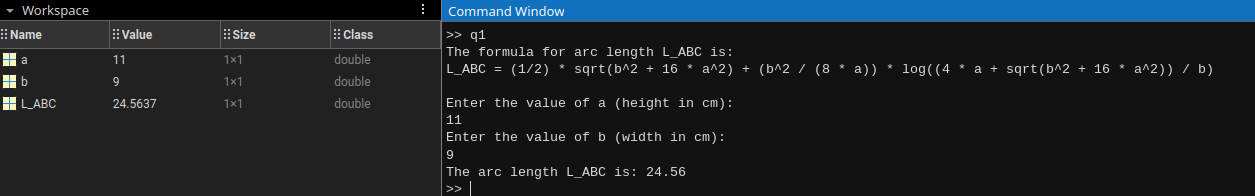
\includegraphics[width=1\textwidth]{images/q1final.png}
    \newpage
    
    
    
    \subsection{Advanced version}

    We are tasked with analyzing a parabola where:\\
    \vspace{1em}
    \hspace{3.8em}
    \begin{minipage}{0.6\textwidth}\centering
        \begin{itemize}[itemsep=-0.1cm]
            \item $a$ represents the height of the parabola
            \item $b$ represents the width of the parabola
        \end{itemize}
    \end{minipage}\\
    \vspace*{1em}
    My goal is to plot the parabola, first by formulating an equation in terms of these factors. Initially, we begin with a simple parabola in the general shape ($x^2$) similar to shown in the question. Our goal is to select a reasonable function, with variables associated with the $x$ scale and $y$ location of the parabola:    
    \[
    y = -(\beta x)^2 + \gamma
    \]
    Given our problem statement:\\
    \vspace{1em}
    \hspace{3.8em}
    \begin{minipage}{0.8\textwidth}\centering
        \begin{itemize}[itemsep=-0.1cm]
            \item $\gamma$ represents the height, so $\gamma = a$
            \item The width is related to the roots of the equation when $y = 0$
        \end{itemize}
    \end{minipage}\\
    \vspace{1em}
    To find $\beta$, we solve:
    \[0 = -(\beta x)^2 + \gamma\]
    \[\beta = \frac{2\sqrt{\gamma}}{b}\]
    since we know $\gamma$:
    \[\beta = \frac{2\sqrt{a}}{b}\]
    Note: This requires $b \neq 0$ and $\sqrt{a} \neq 0$ (i.e., $a > 0$).\\
    Substituting $\gamma$ and $\beta$ into our original equation:
    \[\boxed{y = -\left(\frac{2\sqrt{a}}{b}x\right)^2 + a}\]
    This is our final parabola equation in terms of $a$ and $b$.\\
    \subsection{General Formula for Arc Length}
    In general, the arc length $L$ of a function $f(x)$ from $x_1$ to $x_2$ is given by the formula:
    \[L = \int_{x_1}^{x_2} \sqrt{1 + \left( \frac{d}{dx}(f(x)) \right)^2} \, dx\]
    For our function, we can substitute the derived equation $y = -\left(\frac{2\sqrt{a}}{b}x\right)^2 + a$ into this formula and compute the arc length from $-\frac{b}{2}$ to $\frac{b}{2}$.
    \subsection{Simplification and Resulting Expression}
    After performing the integration, we arrive at the following expression for the arc length:
    \[L = \int_{-\frac{b}{2}}^{\frac{b}{2}} \sqrt{1 + \left(\frac{\partial}{\partial x}\left(-\left(\frac{2\sqrt{a}}{b}x\right)^2 + a\right)\right)^2} \, dx = \frac{4a \sqrt{b^{4} + 16a^{2} b^{2}} + \operatorname{arsinh}\left(\frac{4a}{b}\right) \, b^{3}}{8ab}\]
    This is the arc length of the parabola from $x = -\frac{b}{2}$ to $x = \frac{b}{2}$ for our derived expression.
    \subsection{Comparison of the Two Expressions}
    We now compare this arc length expression with the expression in the question for the length $L_{ABC}$:
    \[L_{ABC} = \frac{1}{2}\sqrt{b^2 + 16a^2} + \frac{b^2}{8a}\ln\left(\frac{4a + \sqrt{b^2 + 16a^2}}{b}\right)\]
    \[L = \frac{4a \sqrt{b^{4} + 16a^{2} b^{2}} + \operatorname{arsinh}\left(\frac{4a}{b}\right) \, b^{3}}{8ab}\]
    Both expressions aim to approximate the arc length of the parabola, they involve different methods of formulation since i didnt get the exact match of an expression. But i aim to make sure my derived expression tries to matches $L_{ABC}$.
    \subsection{matlab code}
    The following matlab code was used to perform the numerical evaluation:
    \lstinputlisting[style=matlab, title=\textbf{\textcolor{\link}{\texttt{\href{https://github.com/sakx7/mathcompuni/blob/main/matlab scripts/expression.m}{matlab scripts/expression.m}}}}]{matlab scripts/expression.m}
    \newpage
    \subsection{Numerical Evaluation}
    Using the python we evaluated both expressions for various values of $a$ and $b$.\\
    The results are summarized in Table
    \begin{table}[H]
        \centering
        \begin{tabular}{|c|c|c|c|c|}
            \hline
            \textbf{a} & \textbf{b} & $\bm{L}$ & $\bm{L_{ABC}}$ & \textbf{Difference} \\
            \hline
            1 & 1 & 2.323392 & 2.323392 & 0.0 \\
            1 & 2 & 2.957886 & 2.957886 & 0.0 \\
            1 & 3 & 3.735939 & 3.735939 & 0.0 \\
            1 & 4 & 4.591174 & 4.591174 & 0.0 \\
            1 & 5 & 5.491150 & 5.491150 & 0.0 \\
            2 & 1 & 4.204658 & 4.204658 & 0.0 \\
            2 & 2 & 4.646784 & 4.646784 & 0.0 \\
            2 & 3 & 5.232421 & 5.232421 & 0.0 \\
            2 & 4 & 5.915771 & 5.915771 & 0.0 \\
            2 & 5 & 6.668527 & 6.668527 & 0.0 \\
            3 & 1 & 6.153288 & 6.153288 & 0.0 \\
            3 & 2 & 6.498059 & 6.498059 & 0.0 \\
            3 & 3 & 6.970176 & 6.970176 & 0.0 \\
            3 & 4 & 7.536853 & 7.536853 & 0.0 \\
            3 & 5 & 8.176498 & 8.176498 & 0.0 \\
            4 & 1 & 8.123944 & 8.123944 & 0.0 \\
            4 & 2 & 8.409317 & 8.409317 & 0.0 \\
            4 & 3 & 8.807604 & 8.807604 & 0.0 \\
            4 & 4 & 9.293568 & 9.293568 & 0.0 \\
            4 & 5 & 9.850171 & 9.850171 & 0.0 \\
            5 & 1 & 10.104730 & 10.104730 & 0.0 \\
            5 & 2 & 10.349698 & 10.349698 & 0.0 \\
            5 & 3 & 10.695939 & 10.695939 & 0.0 \\
            5 & 4 & 11.123014 & 11.123014 & 0.0 \\
            5 & 5 & 11.616959 & 11.616959 & 0.0 \\
            \hline
        \end{tabular}
        \caption{Comparison of $L$ and $L_{ABC}$ with differences}
    \end{table}
        \vspace{-2em}
        
\subsection{Conclusion}
\vspace{1em}

\begin{minipage}{0.45\textwidth}
    The primary objective of this analysis was to derive a function \( f(x) \) whose arc length would graphically correspond to the expression for \( L_{ABC} \) as provided in the question. Initially, the aim was to find a suitable mathematical function that, when graphed, would exhibit the same arc length as that described by \( L_{ABC} \).\\[8pt]
    In pursuit of this goal, we began with a simple parabolic shape and formulated the equation:
    \[y = -\left(\frac{2\sqrt{a}}{b}x\right)^2 + a\]
\end{minipage}\hfil
\begin{minipage}{0.45\textwidth}
    where the parameters \( a \) and \( b \) represent the height and width of the parabola, respectively. This function was chosen because its general form would allow us to manipulate the height and width as required by the problem.\\[8PT]
    To compute the arc length of this parabola, we substituted it into the general formula for arc length:
    \[L = \int_{-\frac{b}{2}}^{\frac{b}{2}} \sqrt{1 + \left( \frac{d}{dx}\left( -\left( \frac{2\sqrt{a}}{b}x \right)^2 + a \right) \right)^2} \, dx\]
\end{minipage}
\newpage

After performing the integration, we derived the following expression for the arc length:
\[L = \frac{4a \sqrt{b^{4} + 16a^{2} b^{2}} + \operatorname{arsinh}\left(\frac{4a}{b}\right) \, b^{3}}{8ab}\]
This derived arc length expression was then compared to the given formula for \( L_{ABC} \):
\[L_{ABC} = \frac{1}{2} \sqrt{b^2 + 16a^2} + \frac{b^2}{8a} \ln \left( \frac{4a + \sqrt{b^2 + 16a^2}}{b} \right)\]
Upon performing numerical evaluations for various values of \( a \) and \( b \), we observed that both arc length expressions provided identical results, with the differences being negligible. The numerical comparison confirmed that the arc length derived from our function matches the given formula for \( L_{ABC} \), thus demonstrating that the function:
\[f(x) = -\left(\frac{2\sqrt{a}}{b}x\right)^2 + a\]
correctly models the desired parabola, and its arc length matches the expression for \( L_{ABC} \) derived from the problem statement.\\
In conclusion, we have successfully achieved the objective of finding a function whose arc length corresponds to the given expression for \( L_{ABC} \). Through rigorous derivation and numerical verification, we have shown that both expressions for the arc length are equivalent. Therefore, we conclude that:
\[L \equiv L_{ABC}\]
This result not only validates the correctness of the derived function but also demonstrates that different methods of obtaining the arc length lead to the same result, confirming the equivalence of the expressions. This completes the analysis and fulfills the original goal set out in the advanced method i aimed to grasp.\\[1em]


    When implementing this in a program:
    \begin{itemize}[itemsep=-0.1cm]
        \item Ensure that when there are no limit parameters for the inputs \(a\) and \(b\), the conditions \(a > 0\) and \(b \neq 0\) are appropriately handled.
        \item Update the plot of \(y = -\left(\frac{2\sqrt{a}}{b}x\right)^2 + a\) so that the sliders for \(a\) and \(b\) directly control the height and width, respectively.
        \item Calculate the arc length of the parabola using the function given the question with inputs \(a\) and \(b\), and display the result in the plot.
    \end{itemize}
    \raggedright
    
    I tried using MATLAB to do this, but it seemed really awkward and unreliable. Although its fine \texttt{.m} version still could require development, but I find that the \texttt{.py} version functions better.

    \newpage
    
    \centering
    
    \href{https://github.com/sakx7/mathcompuni/blob/main/matlab scripts/q1_advanced.m}{\textcolor{\link}{\textbf{matlab scripts/q1\_advanced.m}}}
   
    
    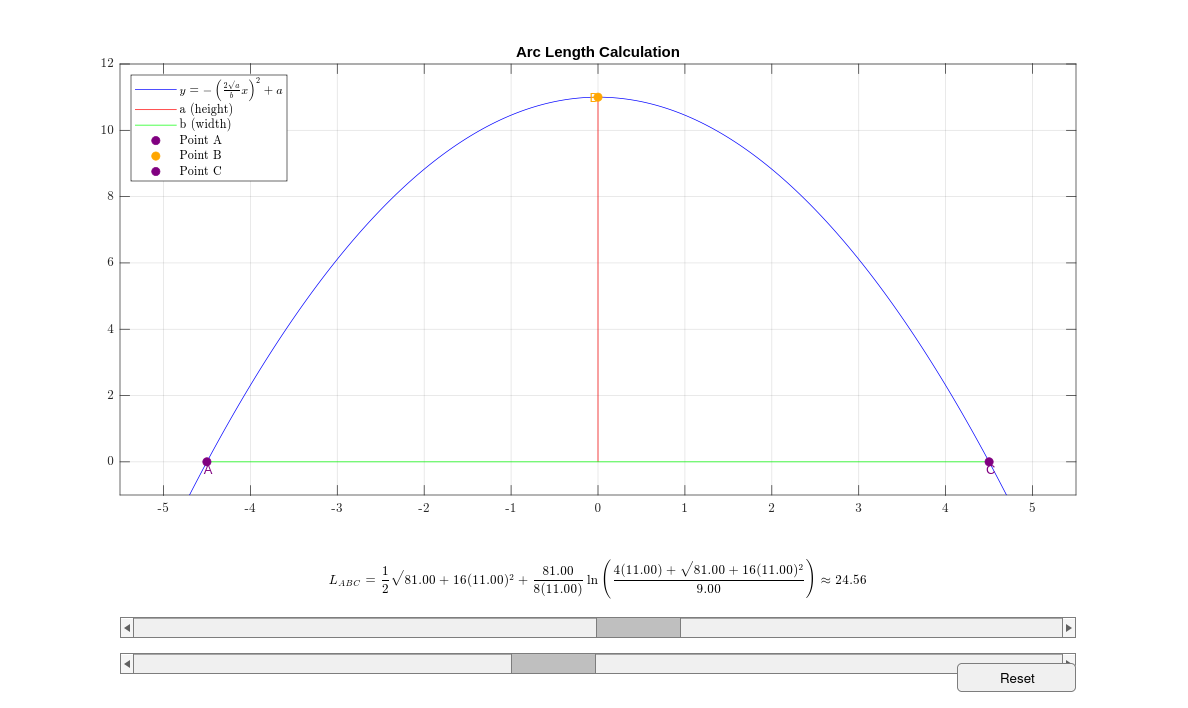
\includegraphics[width=1\textwidth]{images/rmatFigure_1.png}\\
    \vspace{2em}    
    \hrule
    \vspace{3em}
    \href{https://github.com/sakx7/mathcompuni/blob/main/py scripts/q1_advanced.py}{\textcolor{\link}{\textbf{py scripts/q1\_advanced.py}}}
    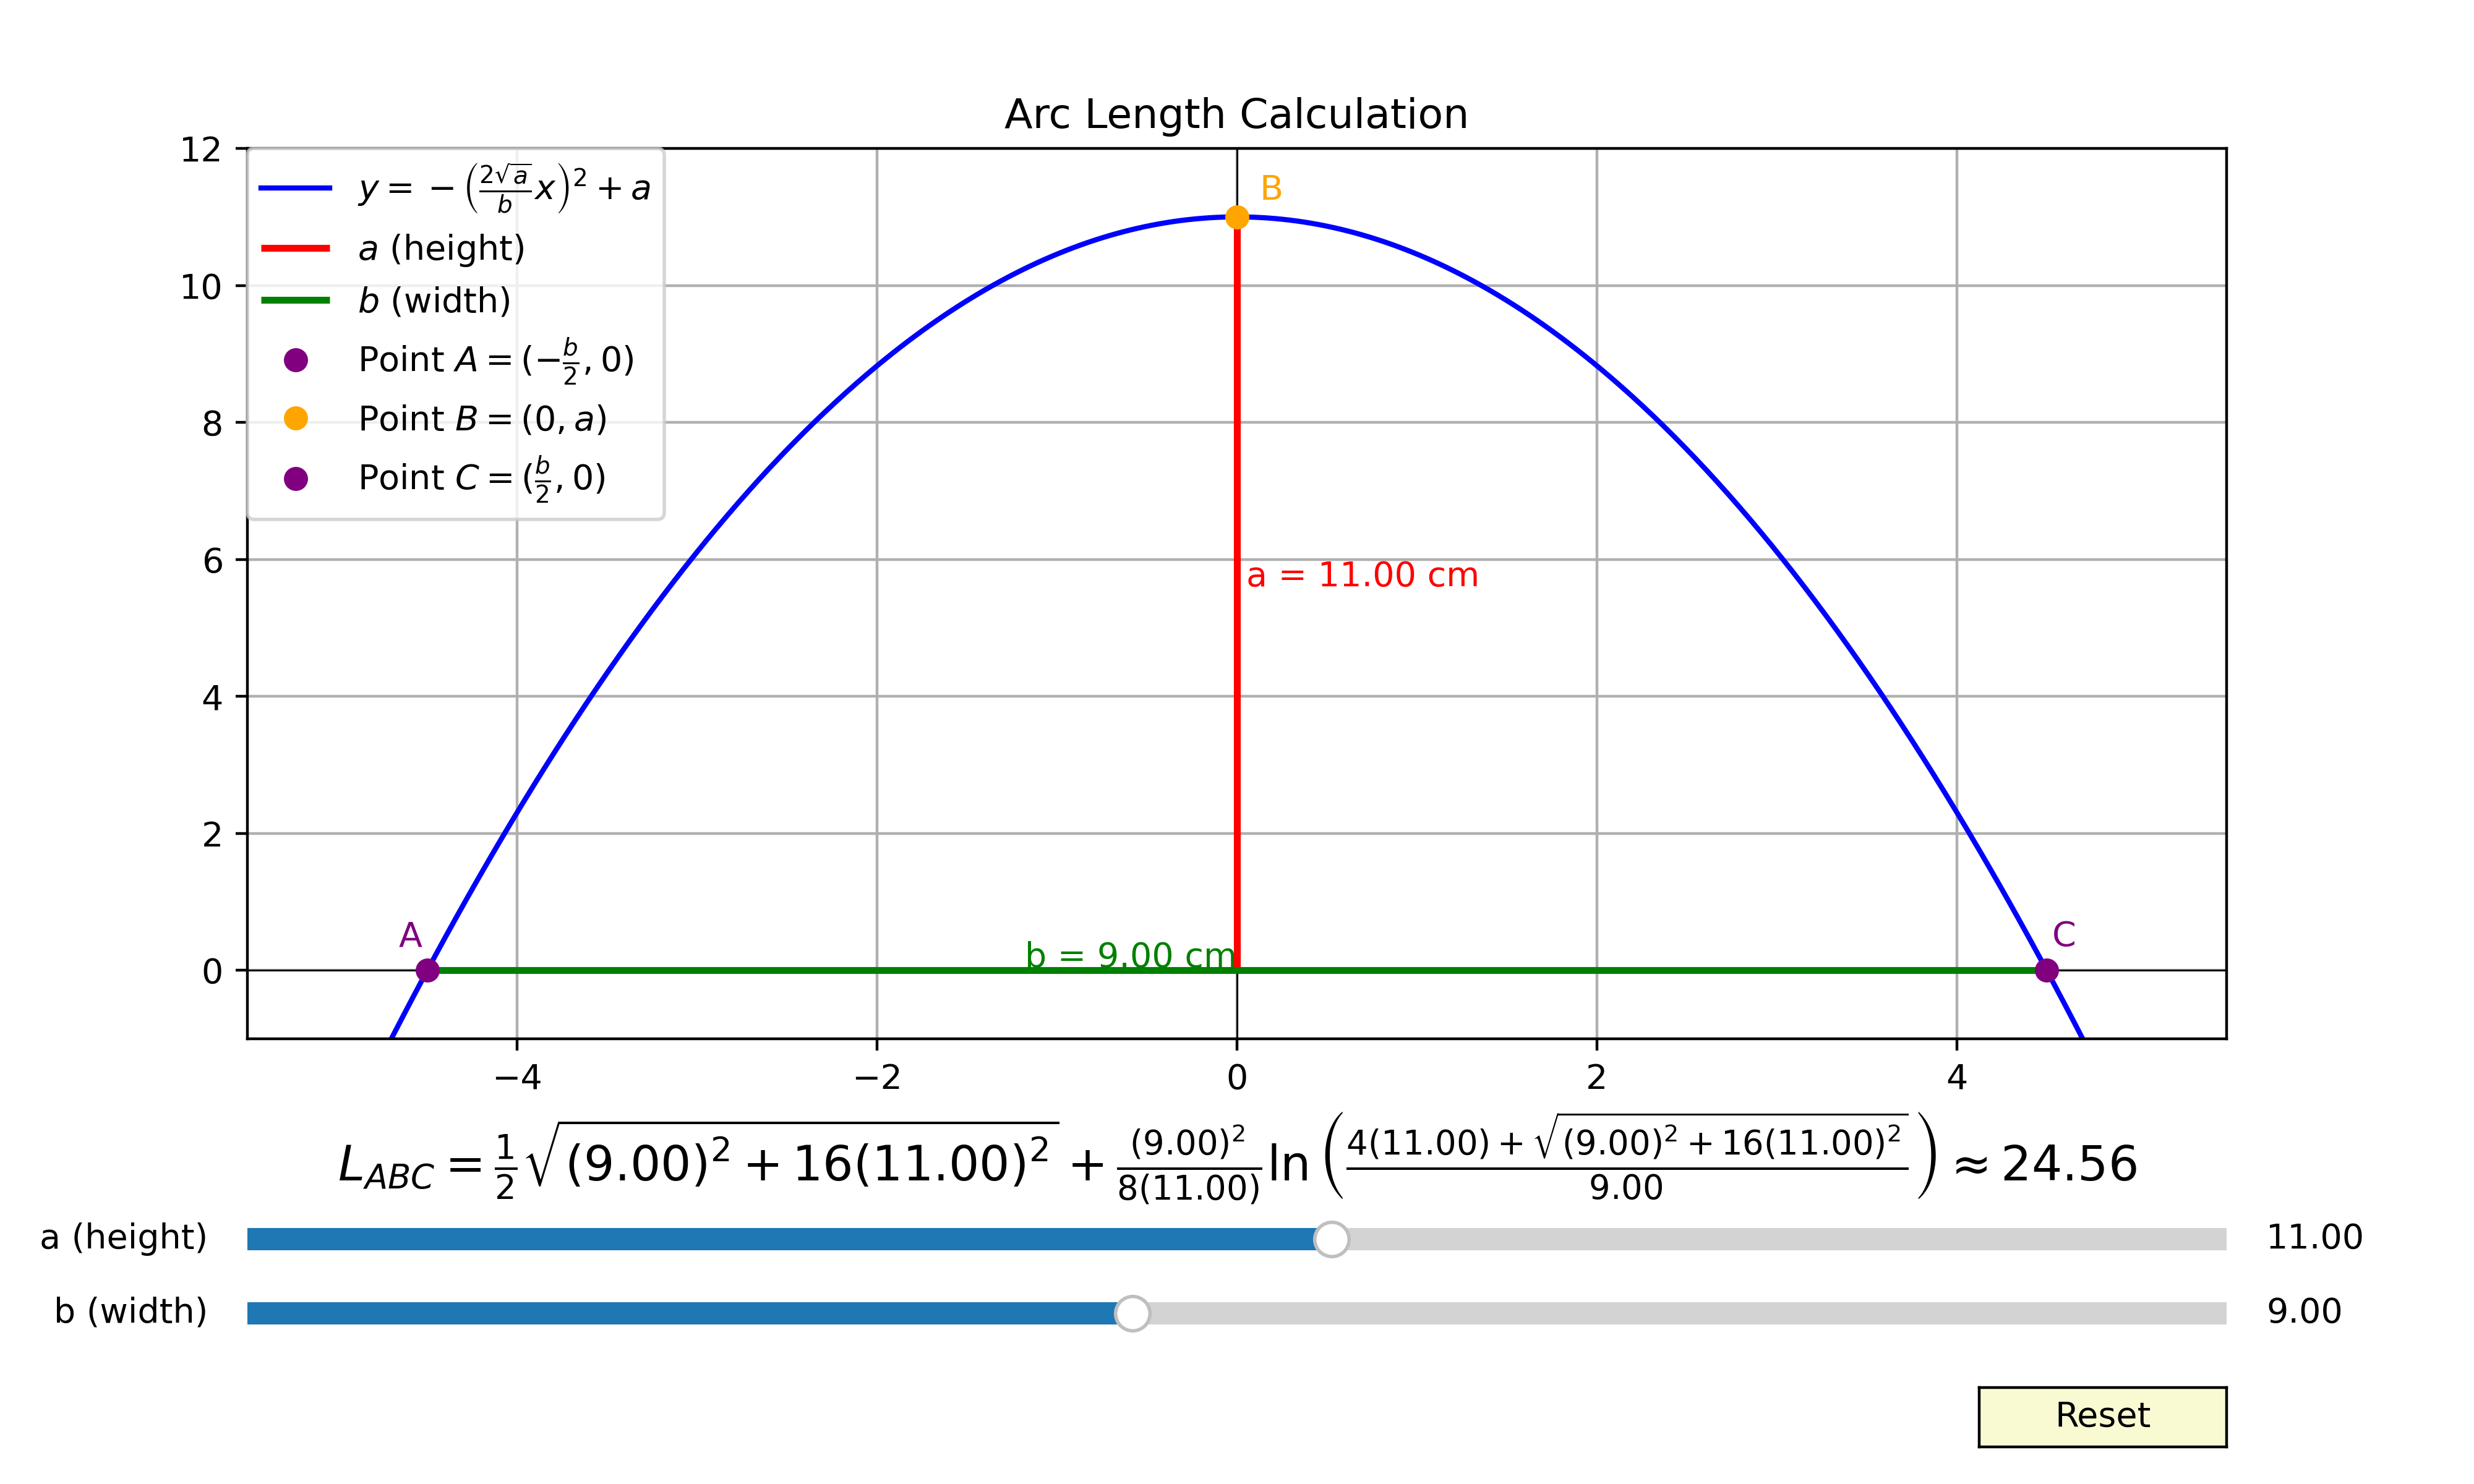
\includegraphics[width=1\textwidth]{images/Figure_1.png}\\
    %\lstinputlisting[style=mypythonstyle,
    %title=\textbf{\textcolor{\link}{\texttt{\href{https://github.com/sakx7/mathcompuni/blob/main/py %scripts/q1_advanced.py}{py scripts/q1\_advanced.py}}}}]{py scripts/q1_advanced.py}

    
   \newpage
   \begin{tcolorbox}[title=\color{black}{\section{Q2}}, colback=white, colframe=\ni, boxrule=1mm, width=1\textwidth]\centering
   The voltage difference \(V_{ab}\) between points \(a\) and \(b\) in the Wheatstone bridge circuit is:
   \[V_{ab} = V \left(\frac{R_1 R_3 - R_2 R_4}{(R_1 + R_2)(R_3 + R_4)}\right)\]
   Write a universal, user-friendly program that calculates the voltage difference \(V_{ab}\).\\    
   Test your program using the following values:\\
   \vspace{1em}
    \begin{minipage}{0.4\textwidth}
    \centering
    \begin{itemize}[itemsep=-0.1cm]
        \item \(V = 14\) volts
        \item \(R_1 = 120.6\ \Omega\)
        \item \(R_2 = 119.3\ \Omega\)
        \item \(R_3 = 121.2\ \Omega\)
        \item \(R_4 = 118.8\ \Omega\)
    \end{itemize}
    \end{minipage}\hspace{-5em}
    \begin{minipage}{0.4\textwidth}
    \begin{circuitikz}[scale=1.3]
        \def\sc{1.3}
        \ctikzset{resistors/zigs=4, resistors/scale=.75,resistors/width=1.3}
        \draw
        node[ocirc] (A) at (2*\sc,0) {} 
        node[ocirc] (B) at (2*\sc,2*\sc) {}
        node[ocirc, label=left:$a$] (C) at (1*\sc,1*\sc) {}
        node[ocirc,label=right:$b$] (D) at (3*\sc,1*\sc) {}
        (A) to[short] (0.3,0) 
        to[american voltage source, v=$V$] (0.3,2*\sc)
        to[short] (B)
        (B) to[R, l_={$R_1$},] (C)
        to[R, l_={$R_2$}] (A)
        (B) to[R, l^={$R_3$}] (D)
        to[R, l^={$R_4$}] (A);
    \end{circuitikz}
\end{minipage}
    
    \end{tcolorbox}

    \lstinputlisting[style=matlab, title=\textbf{\textcolor{\link}{\texttt{\href{https://github.com/sakx7/mathcompuni/blob/main/matlab scripts/q2.m}{matlab scripts/q2.m}}}}]{matlab scripts/q2.m}
    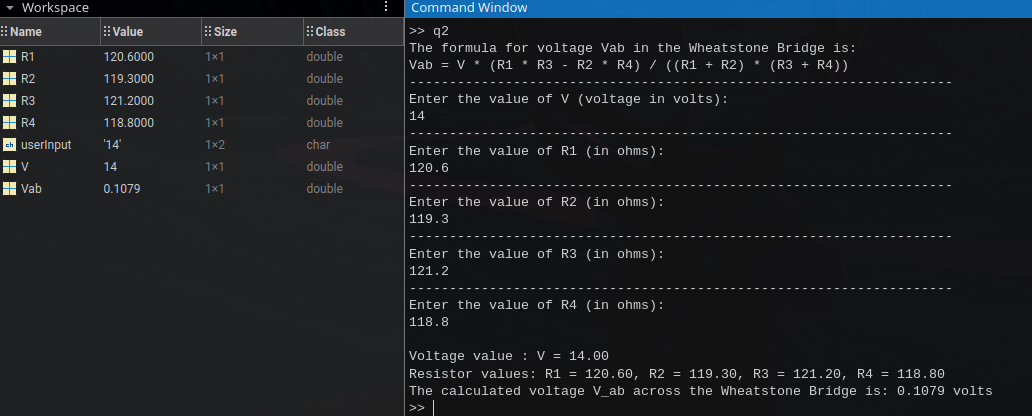
\includegraphics[width=0.9\textwidth]{images/q2f.png}
    \newpage
    
    
    \newpage
    \subsection{Somewhat Advanced Version}
    I say "somewhat" because this isn't all that advanced. One way to improve this project is by incorporate real-time elements, such as allowing users to adjust the resistors while the voltage is still flowing, making it interactive. Ultimately, it’s all about how creative you want to be with this.\\[1em]
    For now, I have developed a nice UI interface in MATLAB, which should suffice. If I have enough time and motivation, I may revisit this and create some animations.\\
    \vspace{1em}
    \href{https://github.com/sakx7/mathcompuni/blob/main/matlab scripts/q2_advanced.m}{\textcolor{\link}{\textbf{matlab scripts/q2\_advanced.m}}}\\[1em]
    
    \begin{center}
        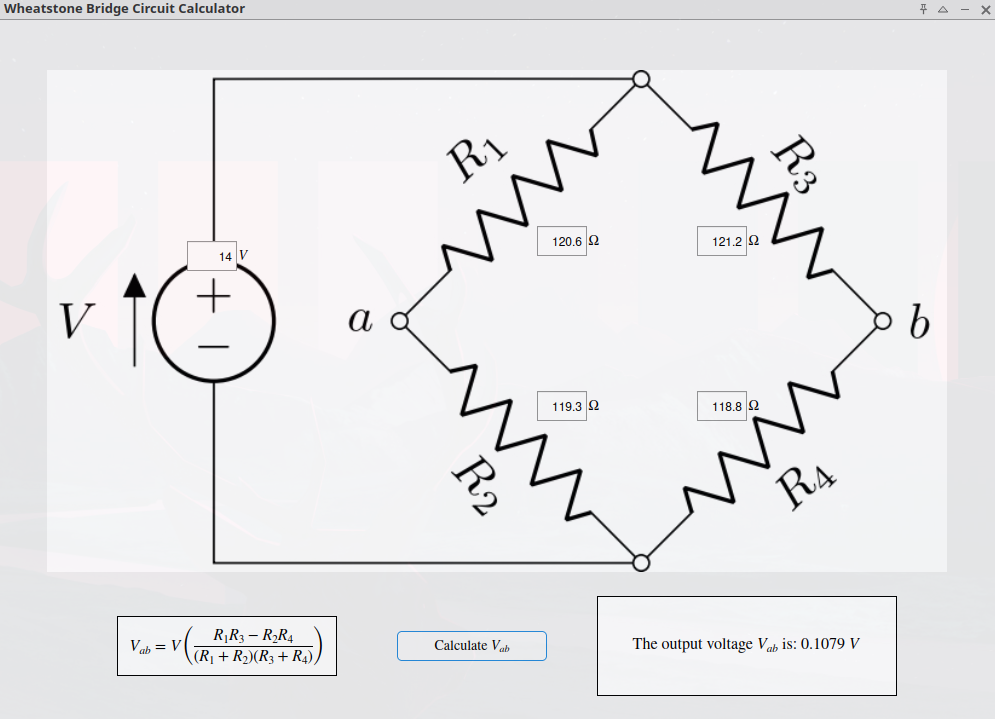
\includegraphics[width=0.9\textwidth]{images/q2a.png}
    \end{center}


    
    \newpage
    \begin{tcolorbox}[title={\color{black}{\section{Q3}}}, colback=white, colframe=\ni, boxrule=1mm, width=1\textwidth]
        \centering
        Newton's law of cooling gives the temperature \( T(t) \) of an object at time \( t \) in terms of \( T_0 \), its temperature at \( t = 0 \), and \( T_s \), the temperature of the surroundings:
        \[
        T(t) = T_s + (T_0 - T_s)e^{-kt}
        \]
        A police officer arrives at a crime scene in a hotel room at 9:18 PM, where he finds a dead body. He immediately measures the body's temperature and finds it to be \( 26.4^\circ C \). Exactly one hour later, he measures the temperature again and finds it to be \( 25.5^\circ C \).\\[6pt]
        Determine the time of death, assuming that the victim's body temperature was normal (\( 36.6^\circ C \)) prior to death, and that the room temperature was constant at \( 20.5^\circ C \).
    \end{tcolorbox}
    
    To solve this problem, I need to fully understand it first before actually importing computing aspects. First, I will use the formula given along with the given information to find the time of death.\\[4pt]
    Let's break it down step by step:\\[1.4em]
    \raggedright
    \begin{minipage}{0.55\textwidth}
        \begin{enumerate}[itemsep=-0.1cm]
            \item \textbf{Finding the cooling constant \( k \)}:
            \begin{itemize}
                \item At 9:18 PM (\( t = 0 \)): \( T_0 = 26.4^\circ C \)
                \item At 10:18 PM (\( t = 1 \) hour): \( T(1) = 25.5^\circ C \)
                \item Room temperature (\( T_s \)) = \( 20.5^\circ C \)
            \end{itemize}
        \end{enumerate}
        \centering
        Using the equation:
        \[ T(t) = T_s + (T_0 - T_s)e^{-kt} \]
        Rearrange for \( k \):
        \[ k = -\frac{1}{t} \ln\left(\frac{T(t) - T_s}{T_0 - T_s}\right) \]
        Plugging in the values:
        \[ k = -\frac{1}{1} \ln\left(\frac{25.5 - 20.5}{26.4 - 20.5}\right) \approx 0.1656 \]
    \end{minipage}\hfill
    \begin{minipage}{0.45\textwidth}
        2. \textbf{Finding the time when \( T_0 = 36.6^\circ C \)}:\\
        Now that we have \( k \), we can use the original equation to find \( t \), rearrange the equation for \( t \):
        \[ t = -\frac{1}{k} \ln\left(\frac{T(t) - T_s}{T_0 - T_s}\right) \]
        Plugging in values and solving for \( t \):
        \[ t = -\frac{1}{0.1656} \ln\left(\frac{25.5 - 20.5}{36.6 - 20.5}\right) \approx 7.06513 \]
    \end{minipage}\\
    \vspace{2em}
    3. \textbf{Calculating the time of death}:\\
    This means the body had been cooling for about \( 7.07 \) hours when the officer arrived at \( 9:18 \) PM. Converting decimal hours into hours and minutes:
    \[ 7 \text{ hr} + 0.07 \times 60 \text{ min} = 7 \text{ hr} + 4.2 \text{ min} \approx 7 \text{ hr} + 4 \text{ min} \]
    To find the time of death, we subtract \( 7 \text{ hr} \) and \( 4 \text{ min} \) from \( 9:18 \) PM:
    \[ 9:18 \text{ PM} - 7 \text{ hr} 4 \text{ min} \approx 2:14 \text{ PM} \]
    Therefore, the estimated time of death is around \textbf{2:14 PM} on the same day.\\[1em]
    \newpage
    \lstinputlisting[style=matlab, title=\textbf{\textcolor{\link}{\texttt{\href{https://github.com/sakx7/mathcompuni/blob/main/matlab scripts/q3.m}{matlab scripts/q3.m}}}}]{matlab scripts/q3.m}
    \centering
    \vspace{1em}
    
    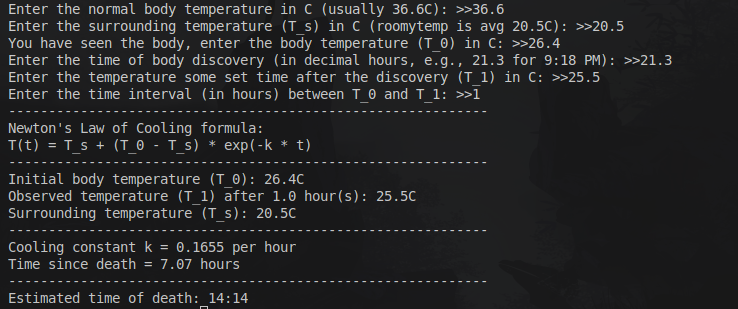
\includegraphics[width=0.8\textwidth]{images/q3.png}
    
    \newpage
    \begin{tcolorbox}[title={\color{black}{\section{Q4}}}, colback=white, colframe=\ni, boxrule=1mm, width=1\textwidth]
        \centering
        The volume of the parallelepiped shown can be calculated by \( \vec{r}_{OB} \cdot (\vec{r}_{OA} \times \vec{r}_{AC}) \).\\
         Use the following steps in a script file to calculate the area:
         \begin{enumerate}[itemsep=-0.1cm]
             \item Define the vectors \( \vec{r}_{OA} \), \( \vec{r}_{OB} \), and \( \vec{r}_{AC} \) from inputted positions of points \( A \), \( B \), and \( C \).
             \item Determine the volume by using MATLAB's built-in functions \texttt{dot} and \texttt{cross}.
         \end{enumerate}
        \tdplotsetmaincoords{70}{110}
        \tdplotsetrotatedcoords{10}{-10}{0}
        \begin{tikzpicture}[tdplot_main_coords, tdplot_rotated_coords, scale=0.5]
            \draw[thick,->] (-9,0,0) -- (15,0,0) node[anchor=north east]{$\bm{x}$};
            \draw[thick,->] (0,-3,0) -- (0,10,0) node[anchor=north west]{$\bm{y}$};
            \draw[thick,->] (0,0,-3) -- (0,0,9) node[anchor=south]{$\bm{z}$};
            \coordinate (O) at (0,0,0);
            \coordinate (A) at (2,5,1);
            \coordinate (B) at (1,3,6);
            \coordinate (C) at (-6,8,2);
            \coordinate (D) at (3,8,7);
            \coordinate (E) at (-8,3,1);
            \coordinate (F) at (-7,6,7);
            \coordinate (G) at (-5,11,8);
            \fill[gray!30, opacity=0.8] (O) -- (A) -- (D) -- (B) -- cycle;
            \fill[gray!30, opacity=0.8] (A) -- (C) -- (G) -- (D) -- cycle;
            \fill[gray!30, opacity=0.8] (B) -- (D) -- (G) -- (F) -- cycle;
            \draw[thick,line width=0.03cm] (O) -- (A) -- (D) -- (B) -- cycle;
            \draw[thick,line width=0.03cm] (A) -- (C) -- (G) -- (D) -- cycle;
            \draw[thick,line width=0.03cm] (B) -- (D) -- (G) -- (F) -- cycle;
            \draw[thick, dashed, dash pattern=on 10pt off 2pt,opacity=0.4] (O) -- (E);
            \draw[thick, dashed, dash pattern=on 10pt off 2pt,opacity=0.4] (E) -- (C);
            \draw[thick, dashed, dash pattern=on 10pt off 2pt,opacity=0.4] (E) -- (F);
            \draw[thick, -{latex[scale=2]}, line width=0.07cm] (A) -- (C) node[midway,below=0.2cm,right=0.1cm] {$\bm{\vec{r}}_{AC}$};
            \draw[thick, -{latex[scale=2]}, line width=0.07cm] (O) -- (A) node[midway,below] {$\bm{\vec{r}}_{OA}$};
            \draw[thick, -{latex[scale=2]}, line width=0.07cm] (O) -- (B) node[midway,above left=-0.2cm] {$\bm{\vec{r}}_{OB}$};
            \node at (O) [above left] {$O$};
            \node at (A) [below=0.2cm, right] {$A(2,5,1)$};
            \node at (B) [above=0.3cm,left=-0.5cm] {$B(1,3,6)$};
            \node at (C) [below=0.2cm, right] {$C(-6,8,2)$};
            \filldraw[white] (O) circle (3pt);
            \filldraw[red] (A) circle (3pt);
            \filldraw[red] (C) circle (3pt);
            \filldraw[red] (B) circle (3pt);
        \end{tikzpicture}
    \end{tcolorbox}
    \lstinputlisting[style=matlab, title=\textbf{\textcolor{\link}{\texttt{\href{https://github.com/sakx7/mathcompuni/blob/main/matlab scripts/q4.m}{matlab scripts/q4.m}}}}]{matlab scripts/q4.m}
    
    \vspace{1em}
    \centering
    
    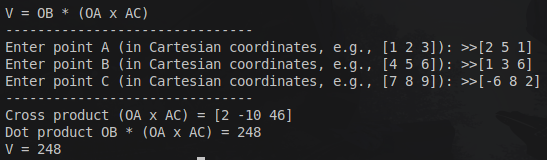
\includegraphics[width=0.6\textwidth]{images/q4.png}
    
    \newpage
    \begin{tcolorbox}[title={\color{black}{\section{Q5}}}, colback=white, colframe=\ni, boxrule=1mm, width=1\textwidth]
        \centering
        The position as a function of time \( (x(t), y(t)) \) of a projectile fired with an initial speed \( v_0 \) at an angle \( \alpha \) is given by:
        \[x(t) = v_0 \cos \alpha \cdot t \qquad y(t) = v_0 \sin \alpha \cdot t - \frac{1}{2} g t^2\]
        where \( g = 9.81 \, \text{m/s}^2 \) is the acceleration due to gravity.\\
        The polar coordinates of the projectile at time \( t \) are \( (r(t), \theta(t)) \), where
        \[r(t) = \sqrt{x(t)^2 + y(t)^2} \qquad \tan \theta(t) = \frac{y(t)}{x(t)}\]
        Write a universal, user-friendly code. Test case: $v_0 = 162$ m/sec and $\alpha = 70^\circ$.\\ Determine $r(t)$ and \(\theta(t)\) for $t = 1, 6, \ldots, 31$ sec.\\
        
            \begin{tikzpicture}[scale=2,transform shape,line width=0.027cm]
            \def\a{2} %main parameter
            \pgfmathsetmacro{\asqrt}{sqrt(\a)}
            
            \fill[bottom color=white, top color=gray] 
            (-\asqrt-0.2, 0) rectangle (\asqrt + 0.3, -0.15);
            
            
            \begin{scope}
                \clip (\asqrt+0.1, 0) rectangle (-\asqrt-0.1, \a+0.1);
                \draw[domain=-\asqrt:\asqrt, samples=100, smooth,dashed] plot (\x, {-(\x)^2 + \a});
            \end{scope}
            
            \draw[-latex] (-\asqrt-0.2, 0) -- (\asqrt+0.5, 0) node[above=-1.6] {\tiny${x}$};
            \draw[-latex] (-\asqrt, 0) -- (-\asqrt, \a+0.5) node[left=-0.1cm] {\tiny${y}$};
            \draw[-latex] (-\asqrt, 0) -- (-\asqrt+0.3, 1) node[left=0.1cm,above=-0.12cm] {\tiny$u$};
            
            \draw[fill=gray!50!white] (0.48, \a-0.225) circle (1pt);
            \draw[fill=gray!50!white] (-\asqrt,0) circle (1pt);
            \draw[-latex] (-1.4142, 0) -- (0.49, 1.787); 
            \node[above] at (-0.4571,0.9) {\tiny$r$};   
            
            \coordinate (O) at (0, 0);
            \coordinate (B) at (-0.4571,0.9);
            \coordinate (A) at (-1.4142, 0);    
            \coordinate (C) at (-1.3, 0.35);
            \coordinate (D) at (-1.3, 0);
            
            \pic [draw, -latex, "\tiny$\theta$", angle eccentricity=1.1,angle radius=1.4cm] {angle = O--A--B};
            \pic [draw, -, "\tiny$\alpha$", angle eccentricity=1.2] {angle = D--A--C};    
        \end{tikzpicture}    
        
    \end{tcolorbox}
    \centering
    Here, I present my past knowledge and comprehension for the equations for projectile motion.
    \renewcommand{\arraystretch}{1.5}
        
    \begin{table}[H]
        \centering
        % First Tabular: Motion Parameters
        \begin{tabular}{|>{\centering\arraybackslash}p{0.3\textwidth}|>{\centering\arraybackslash}p{0.3\textwidth}|>{\centering\arraybackslash}p{0.3\textwidth}|}
            \hline
            \textbf{Parameter} & $\bm{x}$ & $\bm{y}$ \\ \hline
            Acceleration / $a$ & $a_x = 0$ & $a_y = g = 9.81 \, \text{m/s}^2$ \\ \hline
            Initial Velocity / $u$ / $v(0)$ & $u_x = u \cos(\theta)$ & $u_y = u \sin(\theta)$ \\ \hline
            Velocity / $v(t)$ & $v_x(t) = u_x$ & $v_y(t) = u_y - gt$ \\ \hline
            Displacement / $s(t)$ & $s_x(t) = u_x t$ & $s_y(t) = u_y t - \frac{1}{2}gt^2 + h$ \\ \hline
        \end{tabular}
        \vspace{1em}  % Space between sections
        
        % Second Tabular: Time of Flight
        \begin{tabular}{|>{\centering\arraybackslash}p{0.3\textwidth}|>{\centering\arraybackslash}p{0.3\textwidth}|}
            \hline
            Time of Flight / $T$ / $s_y(t)=0$ & $\frac{1}{g}\left(u_y + \sqrt{u_y^2 + 2gh}\right)$ \\ \hline
        \end{tabular}
        \vspace{1em}  % Space between sections
        
        % Third Tabular: Range and Maximum Height Components
        \begin{tabular}{|>{\centering\arraybackslash}p{0.4\textwidth}|>{\centering\arraybackslash}p{0.25\textwidth}|>{\centering\arraybackslash}p{0.25\textwidth}|}
            \hline
            \textbf{Parameter} & $\bm{x}$ & $\bm{y}$ \\ \hline
            Velocity at Separation / $v(T)$ & $v_x(T) = u_x$ & $v_y(T) = \sqrt{u_y^2 + 2gh}$ \\ \hline
            Range / $R$ / \(s_x(T)\)& $\frac{u_x}{g}\left(u_y + \sqrt{u_y^2 + 2gh}\right)$ & $-h$ \\ \hline
            Maximum Height / $H$ / $s(v_y(t)=0)$& \(\frac{u_y u_x}{g}\) & $\frac{u_y^2}{2g} + h$ \\ \hline
        \end{tabular}
        
        \caption{Derivations of Projectile Motion Parameters and Their Component Forms}
        \label{tab:combined_motion_parameters}
    \end{table}
        
        % Table for Circular Motion Parameters
        \begin{table}[H]
            \centering
            \begin{tabular}{|>{\centering\arraybackslash}p{0.3\textwidth}|>{\centering\arraybackslash}p{0.3\textwidth}|}
                \hline
                Radial Position / $r(t)$ & $\sqrt{(s_x(t))^2 + (s_y(t))^2}$ \\ \hline
                Angular Position / $\theta(t)$ & $\tan^{-1}\left(\frac{s_y(t)}{s_x(t)}\right)$ \\ \hline
                Angular Velocity / $\omega(t)$ & $\frac{d}{dt}(\theta(t))$ \\ \hline
                Angular Acceleration / $\alpha(t)$ & $\frac{d}{dt}(\omega(t))$ \\ \hline
            \end{tabular}
            \caption{Circular Motion}
            \label{tab:circular_motion}
        \end{table}
       
        
        % Table for Non-Drag Energy Components
        \begin{table}[H]
            \centering
            \begin{tabular}{|>{\centering\arraybackslash}p{0.3\textwidth}|>{\centering\arraybackslash}p{0.3\textwidth}|>{\centering\arraybackslash}p{0.3\textwidth}|}
                \hline
                Energy Component & $x$ & $y$ \\ \hline
                Kinetic Energy (KE) & $\frac{1}{2}m u_x^2$ & $\frac{1}{2}m u_y^2$ \\ \hline
                Potential Energy (PE) & 0 & $mgh$ \\ \hline
                Total Energy (TE) & $\frac{1}{2}m u_x^2$ & $\frac{1}{2}m u_y^2 + mgh$ \\ \hline
                Lagrangian / $\mathscr{L}$ & $\frac{1}{2}m u_x^2$ & $\frac{1}{2}m u_y^2 - mgh$ \\ \hline
                Power (P) & $m a_x u_x = 0$ & $m a_y u_y = m g u_y$ \\ \hline
                Work Done (W) & 0 & $mgh$ \\ \hline
            \end{tabular}
            \caption{Energy Components in Projectile Motion (Non-Drag)}
            \label{tab:non_drag_energy}
        \end{table}
        
        \vspace{1em}
        
    I will not be implementing drag components (air-resistance), as they are complex and at this point i know i am doing more than what the question asks. In so I will focus solely on the motion parameters rather than energy quantities in the script.\\[2em]
    \lstinputlisting[style=matlab, title=\textbf{\textcolor{\link}{\texttt{\href{https://github.com/sakx7/mathcompuni/blob/main/matlab scripts/q5.m}{matlab scripts/q5.m}}}}]{matlab scripts/q5.m}

    \includegraphics[width=1\textwidth]{images/Projectile_motion.png}
    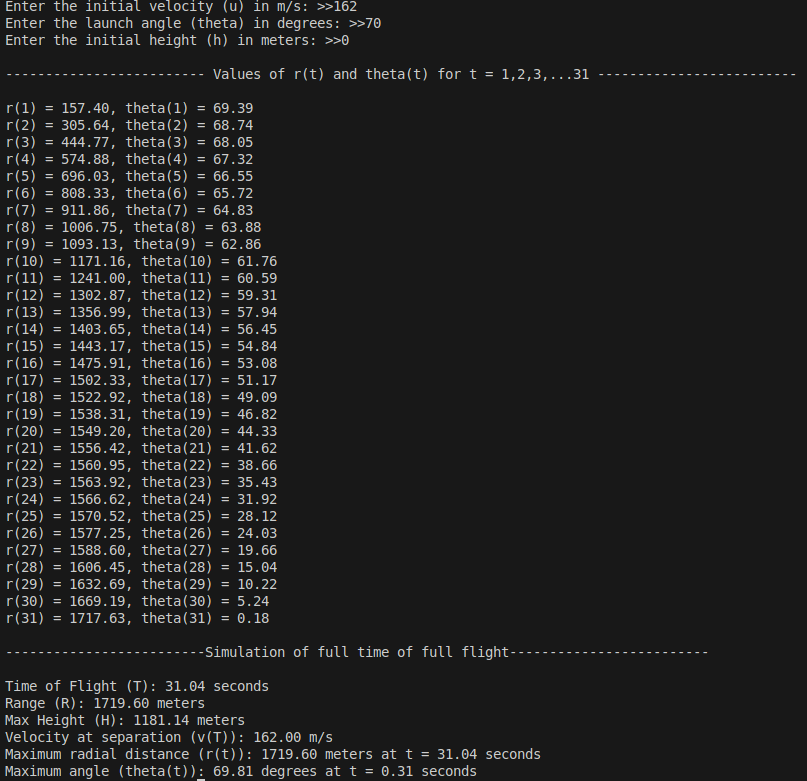
\includegraphics[width=1\textwidth]{images/q5cmd.png}
    
    \newpage
    \begin{tcolorbox}[title={\color{black}{\section{Q6}}}, colback=white, colframe=\ni, boxrule=1mm, width=1\textwidth]
    \centering
    The ideal gas equation states that
    \[P = \frac{nRT}{V}\]
    where \( P \) is the pressure, \( V \) is the volume, \( T \) is the temperature, \( R = 0.08206 \, \text{(L atm)/(mol K)} \) is the gas constant, and \( n \) is the number of moles. Real gases, especially at high pressure, deviate from this behavior. Their response can be modeled with the van der Waals equation
    \[P = \frac{nRT}{V - nb} - \frac{n^2 a}{V^2}\]
    where \( a \) and \( b \) are material constants. Consider 1 mole (\( n = 1 \)) of nitrogen gas at \( T = 300 \, \text{K} \). (For nitrogen gas \( a = 1.39 \, \text{(L}^2 \text{ atm)/mol}^2 \) and \( b = 0.0391 \, \text{L/mol} \).)
    Create a vector with valu3es of \( V \) for \( 0.1 \leq V \leq 1 \, \text{L} \), using increments of \( 0.02 \, \text{L} \). Using this vector, calculate \( P \) twice for each value of \( V \): once using the ideal gas equation and once with the van der Waals equation. Using the two sets of values for \( P \), calculate the percent error
    \[\left( \frac{P_{\text{ideal}} - P_{\text{waals}}}{P_{\text{waals}}} \right) \times 100\]
    for each value of \( V \). Finally, by using MATLAB's built-in function \texttt{max}, determine the maximum error and the corresponding volume.
    \end{tcolorbox}
    \lstinputlisting[style=matlab, title=\textbf{\textcolor{\link}{\texttt{\href{https://github.com/sakx7/mathcompuni/blob/main/matlab scripts/q6.m}{matlab scripts/q6.m}}}}]{matlab scripts/q6.m}
    
    \includegraphics[width=1\textwidth]{images/pressurevolume.png}
    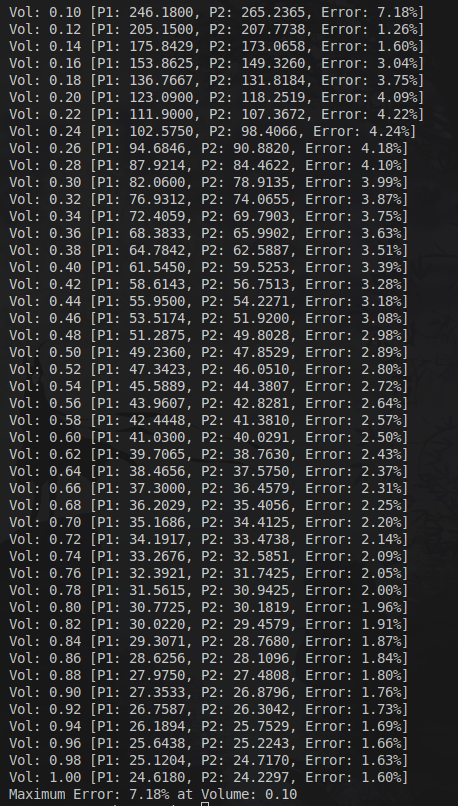
\includegraphics[width=0.6\textwidth]{images/q6.png}
    
    \newpage\newgeometry{margin=1in,left=0.6in,right=0.6in,bottom=0.2in}
    \begin{tcolorbox}[title={\color{black}{\section{Q7}}}, colback=white, colframe=\ni, boxrule=1mm, width=1\textwidth]
         A student has a summer job as a lifeguard at the beach.\\[8pt]
         After spotting a swimmer in trouble, they try to determine the path that will allow them to reach the swimmer in the shortest time.\\[1em] 
         \begin{minipage}{0.45\textwidth} 
            With the lifeguard being able to run faster than they can swim, the path of shortest distance, \textbf{Path A}, is obviously not ideal because it maximises the time spent swimming \(A_w\).\\[8pt]
            Although \textbf{Path B} reduces the amount of time spent swimming \(B_w\), it is probably not the best option because it is the longest feasible path.\\[8pt]
            Therefore, somewhere in between Paths A and B is the best course of action.
         \end{minipage}
         \begin{minipage}{0.4\textwidth}\centering
             \begin{tikzpicture}[scale=1.5,transform shape]
                 \definecolor{sandy}{HTML}{FFFFFF}
                 \definecolor{sea}{HTML}{f8f8f8}
                 \definecolor{news}{HTML}{FFFFFF}
                 \definecolor{seas}{HTML}{f8f8f8}
                 \fill[sandy] (-0.5, -0.5) rectangle (2.5, 3.5);
                 \fill[sea] (2.5, -0.5) rectangle (5.5, 3.5);
                 \draw (2.5, -0.5) -- (2.5, 3.5);
                 \coordinate (D) at (2.5,2.25);    
                 \coordinate (A1) at (2.5,1.5);
                 \coordinate (B) at (5,3);    
                 \coordinate (A) at (0,0);
                 \coordinate (C) at (2.5,3);    
                 \draw[fill=white] (A) circle (2pt) node[below] {\scalebox{0.9}{\sffamily\tiny Lifeguard}};
                 \draw[fill=white] (B) circle (2pt) node[below] {\scalebox{0.9}{\sffamily\tiny Swimmer}};
                 %A
                 \draw[dashed,red] (A) -- (A1);
                 \filldraw[news] (1.25,0.75) circle (0.2cm);
                 \node at (1.25,0.75) {\tiny$A_s$};
                 \draw[dashed,red!70!black,dash pattern=on 3pt off 1pt,opacity=0.6] (A1) -- (B);
                 \filldraw[seas] (3.75,2.25) circle (0.2cm);
                 \node at (3.75,2.25) {\tiny$A_w$};
                 %B
                 \draw[dashed,blue] (A) -- (C);
                 \filldraw[news] (1.25,1.5) circle (0.2cm);
                 \node at (1.25,1.5) {\tiny$B_s$};
                 \draw[dashed,blue!70!black,dash pattern=on 3pt off 1pt,opacity=0.6] (C) -- (B);
                 \filldraw[seas] (3.75,3) circle (0.2cm);
                 \node at (3.75,3) {\tiny$B_w$};
                 %C
                 \draw[-,green] (A) -- (D);
                 \filldraw[news] (1.25,1.125) circle (0.2cm);
                 \node at (1.25,1.125) {\tiny$C_s$};
                 \draw[-,green!70!black] (D) -- (B);    
                 \filldraw[seas] (3.75,2.625) circle (0.2cm);
                 \node at (3.75,2.625) {\tiny$C_w$};
                 \coordinate (phi) at (1.25,2.25);
                 \coordinate (alpha) at (3.75,2.25);
                 \draw[-,gray!70!black,line width=0.001cm] (1.5,2.25) -- (3.5,2.25);
                 \begin{scope}[shift={(0.2,0)}]        
                     \draw[latex-latex,gray!70!black,line width=0.001cm] (2.5,0) -- (2.5,2.25);
                     \filldraw[seas] (2.5,1.125) circle (0.1cm);
                     \node at (2.5,1.125) {\tiny$y$};
                 \end{scope}
                 \draw[-,gray!70!black,line width=0.001cm] (1.5,0) -- (3.5,0);
                 \coordinate (L) at (0,3);
                 \draw[gray!70!black, latex-latex,line width=0.001cm] (A) -- (L);
                 \filldraw[news] (0,1.5) circle (0.16cm);
                 \node at (0,1.5) {\tiny$L$};
                 \draw[gray!70!black, latex-latex,line width=0.001cm] (L) -- (C);
                 \filldraw[news] (1.25,3) circle (0.16cm);
                 \node at (1.25,3) {\tiny$d_s$};
                 \draw[latex-latex,line width=0.001cm,gray!70!black] ([shift={(0, 0.3)}]C) -- ([shift={(0, 0.3)}]B);
                 \filldraw[seas] (3.75,3.3) circle (0.16cm);
                 \node at (3.75,3.3) {\tiny$d_w$};
                 \pic [draw, -{Latex[length=0.5mm,width=0.55mm]}, "\tiny$\phi$", angle eccentricity=1.4,angle radius=0.3cm] {angle = phi--D--A};
                 \pic [draw, -{Latex[length=0.5mm,width=0.55mm]}, "\tiny$\alpha$", angle eccentricity=1.35,angle radius=0.4cm] {angle = alpha--D--B};    
             \end{tikzpicture}
         \end{minipage}\\
         
         \vspace{0.6em}
             
         Consider the intermediate \textbf{path C} consisting of $C_s$ and $C_w$ and determine the time required to reach the swimmer in terms of the following:\\[1em]
         \begin{minipage}{0.4\textwidth}
         \begin{itemize}[itemsep=-0.1cm]
             \item Running speed: \( v_{\text{run}} = 3 \, \text{m/s} \)
             \item Swimming speed: \( v_{\text{swim}} = 1 \, \text{m/s} \)
             \item Distance \( L = 48 \, \text{m} \)
             \item Distance \( d_s = 30 \, \text{m} \)
             \item Distance \( d_w = 42 \, \text{m} \)
             \item Lateral distance \( y \) at which the lifeguard enters the water.
         \end{itemize}
        \end{minipage}\hfil
        \begin{minipage}{0.52\textwidth}
         Create a vector \( y \) that ranges between path A and path B (\( y = 20, 21, 22, \dots, 48 \, \text{m} \)) and compute a time \( t \) for each \( y \).\\[8pt]
         Use MATLAB's built-in function \texttt{min} to find the minimum time and the entry point \( y \) for which it occurs.
        \end{minipage}\\[1em]
        
         Determine the angles that correspond to the calculated value of \( y \) and investigate 
         whether your result satisfies Snell's law of refraction:
         \[\frac{\sin \phi}{\sin \alpha} = \frac{v_{\text{run}}}{v_{\text{swim}}}\]
    \end{tcolorbox}
    The total time \( t \) to reach the swimmer has two parts:\\[8pt]
    
    \begin{minipage}{0.47\textwidth}
        \textbf{1. Running Time}: The running distance \( C_s \) from the starting point to the shore is based on the vertical distance \( y \) and horizontal distance \( d_s \):
        \[
        C_s = \sqrt{y^2 + d_s^2}
        \]
        Thus, the running time is:
        \[
        t_{\text{run}} = \frac{C_s}{v_{\text{run}}} = \frac{\sqrt{y^2 + d_s^2}}{v_{\text{run}}}
        \]
    \end{minipage}
    \hfill
    \begin{minipage}{0.485\textwidth}    
        \textbf{2. Swimming Time}: After reaching \( y \), the lifeguard swims directly to the swimmer. The swimming distance \( C_w \) is based on the horizontal distance \( L - y \) and the vertical distance \( d_s \):
        \[
        C_w = \sqrt{d_s^2 + (L - y)^2}
        \]
        Thus, the swimming time is:
        \[
        t_{\text{swim}} = \frac{C_w}{v_{\text{swim}}} = \frac{\sqrt{d_s^2 + (L - y)^2}}{v_{\text{swim}}}
        \]
    \end{minipage}\\[1em]
   
    Alternatively, \( C_w \) can be related to another triangle involving \( d_w \), the swimmer’s horizontal distance from the shore.

    
    \textbf{3. Total Time} Combining both components, the total time \( t \) required to reach the swimmer is:
    \[ t = t_{\text{run}} + t_{\text{swim}} = \frac{\sqrt{y^2 + d_s^2}}{v_{\text{run}}} + \frac{\sqrt{d_s^2 + (L - y)^2}}{v_{\text{swim}}} \]
    Substituting the known values, we have:
    \[ t = \frac{\sqrt{y^2 + 30^2}}{3} + \frac{\sqrt{30^2 + (48 - y)^2}}{1} \]
    \textbf{Angles for verification with Snells law}
    \[\frac{\sin \phi}{\sin \alpha} = \frac{v_{\text{run}}}{v_{\text{swim}}}\]
    were:
    \[\phi = \arctan\left(\frac{y}{d_s}\right) = \arctan\left(\frac{y}{30}\right)\]
    \[\alpha = \arctan\left(\frac{L-y}{d_s}\right) = \arctan\left(\frac{48-y}{30}\right)\]
    Worked out through observation of triangles formed\\[1em]
    \textbf{Finding the Optimal Path}\\[8pt]
    To find the optimal entry point \( y \) that minimizes \( t \), we compute the time \( t \) for each possible \( y \) within the range of \( 20 \leq y \leq 48 \) m. The entry point \( y \) that yields the minimum time will be our optimal path.\\[1em]
    To solve this problem in code, we:
    \begin{enumerate}[itemsep=-0.1cm]
        \item Define the running and swimming speeds, as well as distances along and perpendicular to the shore.
        \item Use the distance \( y \) as a variable representing where the lifeguard enters the water.
        \item Calculate the total time \( t \) required to reach the swimmer for each \( y \) value.
        \item Use MATLAB’s \texttt{min} function to find the optimal \( y \) with minimum time.
        \item Verify the result with Snell's law.
    \end{enumerate}
    
    \lstinputlisting[style=matlab, title=\textbf{\textcolor{\link}{\texttt{\href{https://github.com/sakx7/mathcompuni/blob/main/matlab scripts/q7.m}{matlab scripts/q7.m}}}}]{matlab scripts/q7.m}
    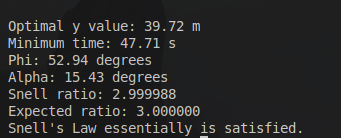
\includegraphics[width=0.5\textwidth]{images/q7.png}

    \newpage
    \begin{tcolorbox}[title={\color{black}{\section{Q8}}}, colback=white, colframe=\ni, boxrule=1mm, width=1\textwidth]    
    In a typical tension test, a dog bone-shaped specimen is pulled in a machine. During the test, the force needed to pull the specimen and the length \( L \) of a gauge section are measured. This data is used for plotting a stress-strain diagram of the material.\\[8pt]
    Two definitions, engineering and true, exist for stress and strain.\\
    The engineering stress \( \sigma_c \) and strain \( \varepsilon_c \) are defined by:\\[0em]
    \[\sigma_c = \frac{F}{A_0} \qquad \varepsilon_c = \frac{L - L_0}{L_0}\]\\[0em]
    where \( L_0 \) and \( A_0 \) are the initial gauge length and the initial cross-sectional area of the specimen, respectively.\\[8pt]
    The true stress \( \sigma_t \) and strain \( \varepsilon_t \) are defined by\\[1em]
    \[\hspace{-8em} \sigma_t = \frac{F L_0}{A_0 L} \qquad \varepsilon_t = \ln\left(\frac{L}{L_0}\right)\]\\
    
    \centering
    \begin{minipage}{0.7\textwidth}    \vspace{-2em}
        The following are measurements of force and gauge length from a tension test with an aluminium specimen.\\[1em]
        The specimen has a round cross-section with a radius of \( 6.4 \, \text{mm} \) (before the test). \\[1em]
        The initial gauge length is \( L_0 = 25 \, \text{mm} \).\\[1em]
        Use the data to calculate and generate the engineering and true stress-strain curves, both on the same plot.\\[1em]
        Label the axes and use a legend to identify the curves.\\[1em]
        \textbf{Units}: When the force is measured in newtons (N) and the area is calculated in m\(^2\), the unit of the stress is pascals (Pa).
    \end{minipage}\hfill
    \begin{minipage}{0.25\textwidth}\vspace{-9em}
    \begin{center}
        \begin{tabular}{|c|c|}
            \hline
            \text{F, N} & \text{L, mm} \\
            \hline
            0 & 25.400 \\
            13.031 & 25.474 \\
            21.485 & 25.515 \\
            31.3963 & 25.575 \\
            34.727 & 25.615 \\
            37.119 & 25.693 \\
            37.960 & 25.752 \\
            39.550 & 25.978 \\
            40.758 & 26.419 \\
            40.986 & 26.502 \\
            41.076 & 26.600 \\
            41.255 & 26.728 \\
            41.481 & 27.130 \\
            41.564 & 27.441 \\
            \hline
        \end{tabular}
    \end{center}
    \end{minipage}
    
    \end{tcolorbox}
    
    \lstinputlisting[style=matlab, title=\textbf{\textcolor{\link}{\texttt{\href{https://github.com/sakx7/mathcompuni/blob/main/matlab scripts/q8.m}{matlab scripts/q8.m}}}}]{matlab scripts/q8.m}
    \vspace{1em}
    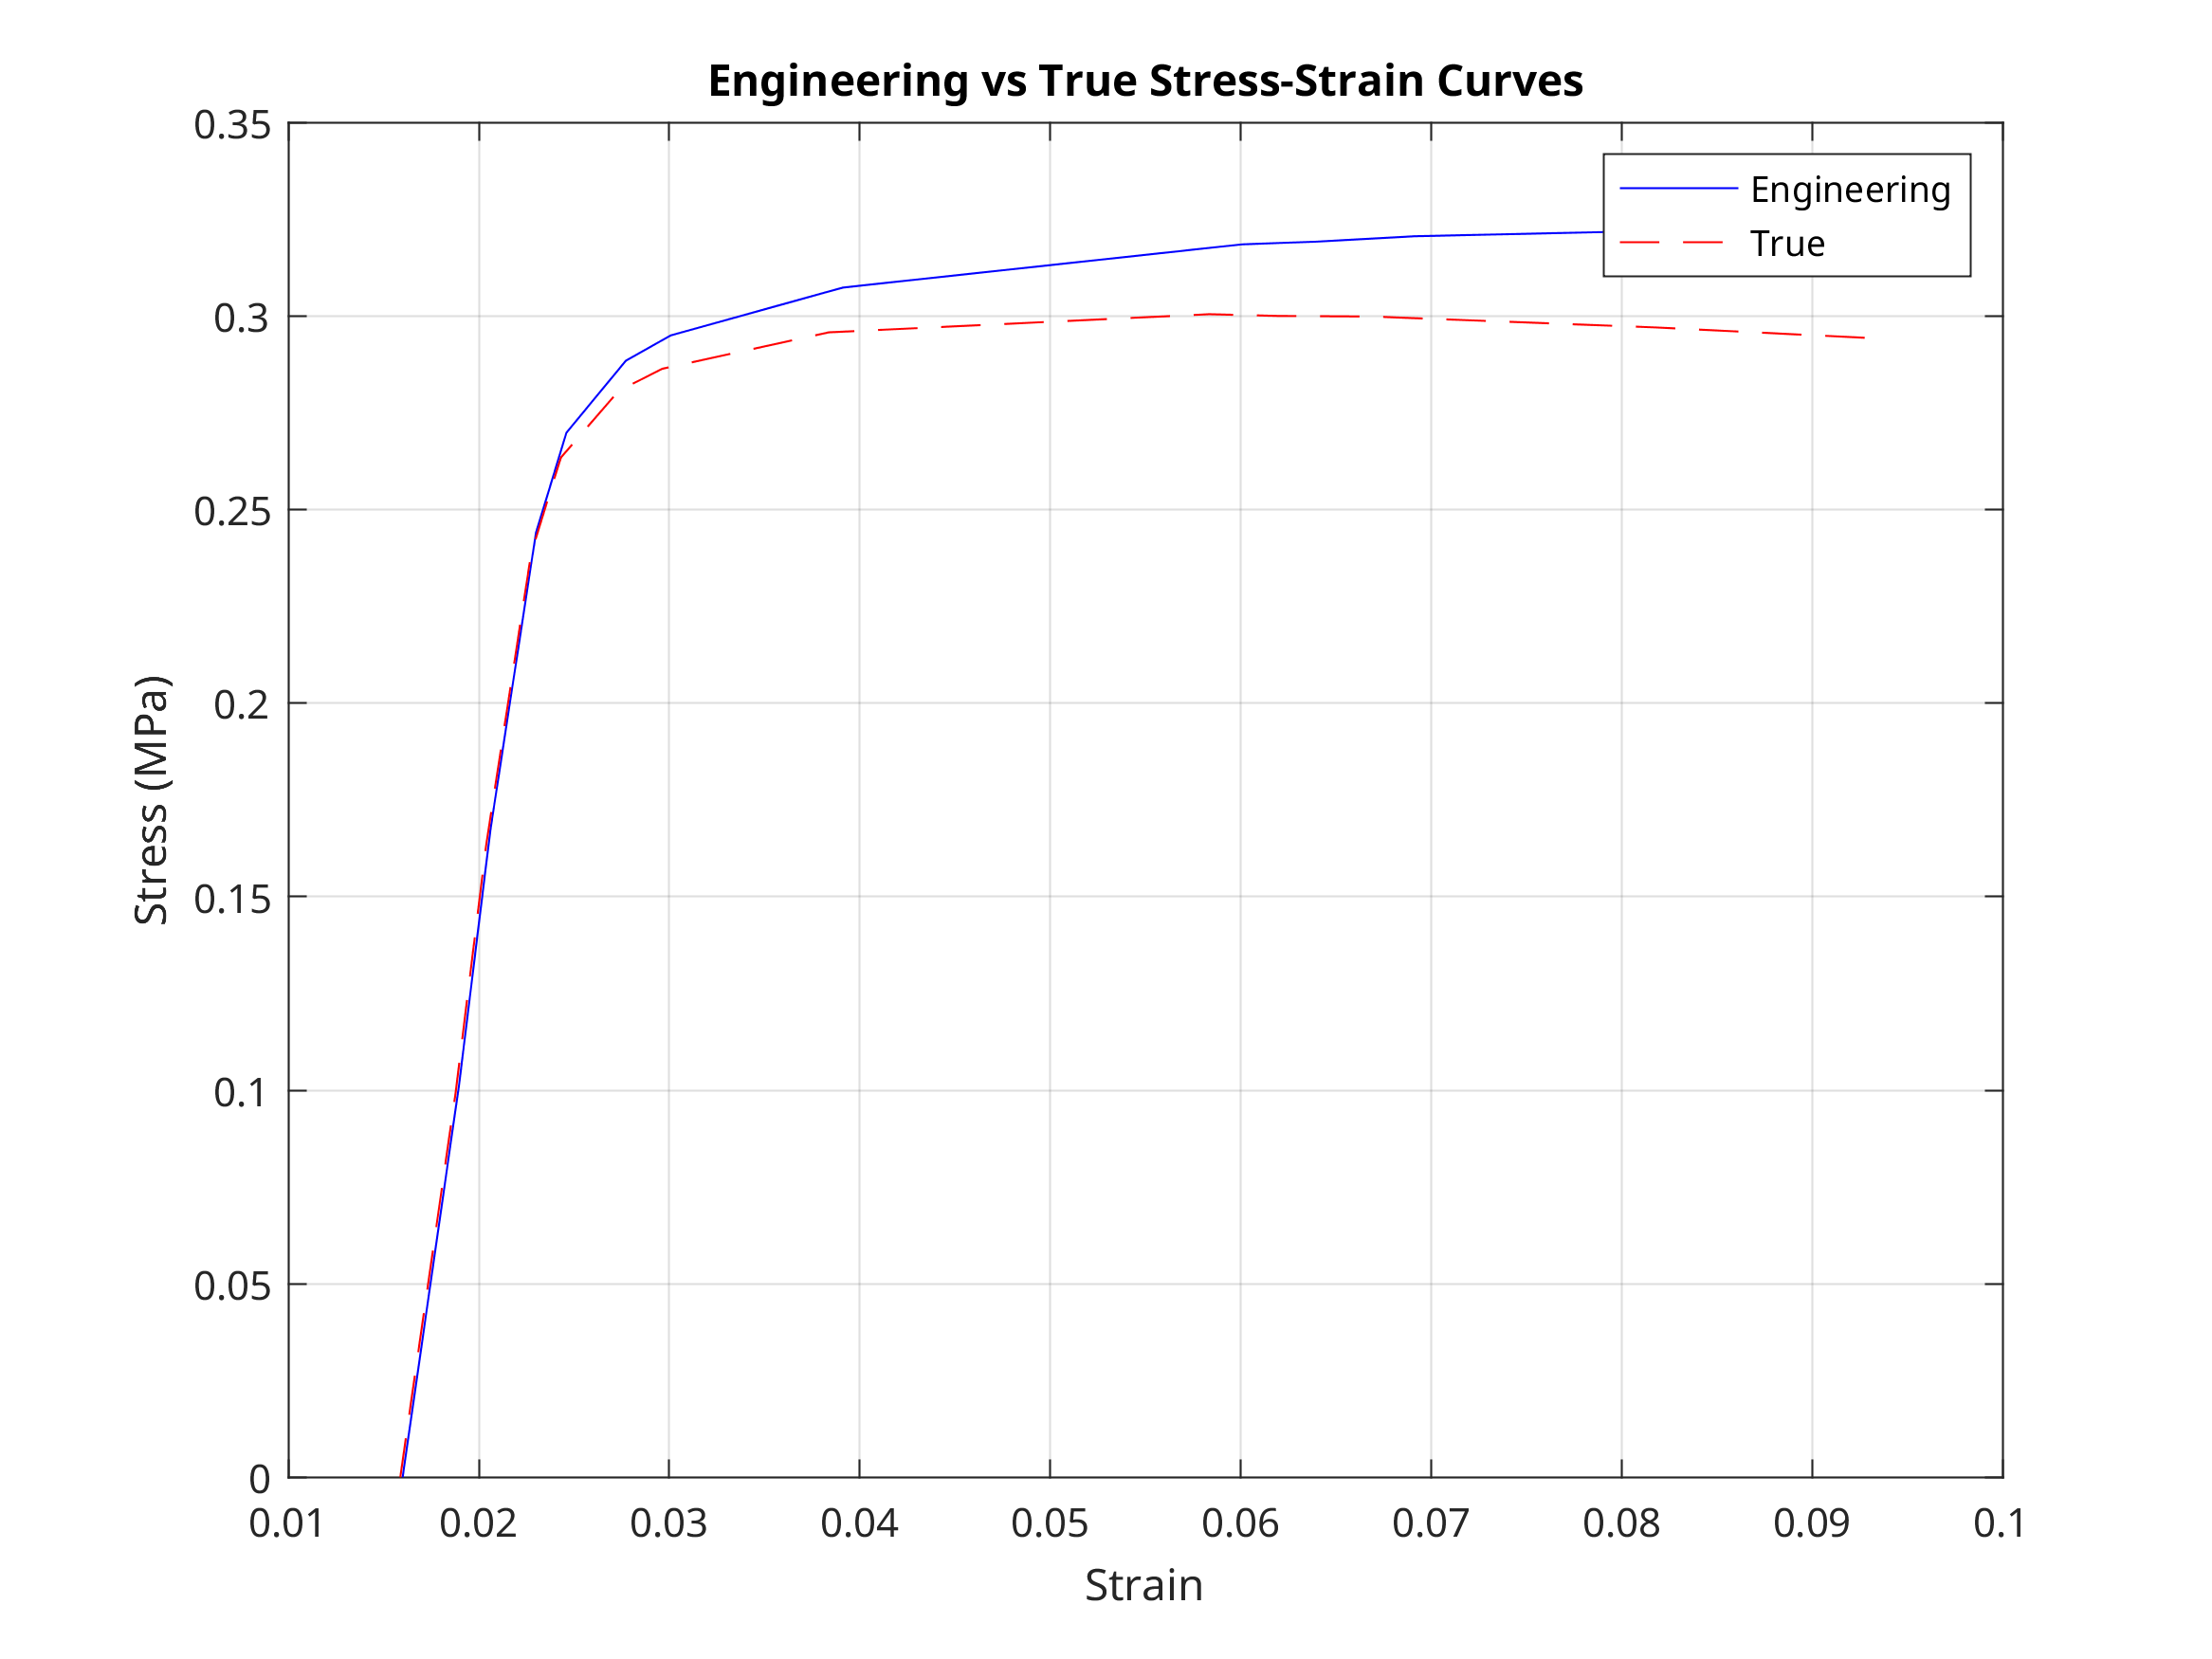
\includegraphics[width=1\textwidth]{images/stressvstran.png}
    \newpage
    
    \begin{tcolorbox}[title={\color{black}{\section{Q9}}}, colback=white, colframe=\ni, boxrule=1mm, width=1\textwidth]    
    A railroad bumper is designed to slow down a rapidly moving railroad car. After a \(20,000 \, \text{kg}\) railroad car traveling at \(20 \, \text{m/s}\) engages the bumper, its displacement \(x\) (in meters) and velocity \(v\) (in m/s) as a function of time \(t\) (in seconds) is given by:
    \[x(t) = 4.219(e^{-1.58t} - e^{-6.32t}) \]
    \centering
    and 
    
    \raggedright
    \[v(t) = 26.67 e^{-6.32t} - 6.67 e^{-1.58t}\]
    Plot the displacement and the velocity as a function of time for \(0 \leq t \leq 4\) seconds. Fit two plots at the top of the window and a plot of both with two vertical axes underneath them. All plots must be of printing quality.
    \end{tcolorbox}
    \lstinputlisting[style=matlab, title=\textbf{\textcolor{\link}{\texttt{\href{https://github.com/sakx7/mathcompuni/blob/main/matlab scripts/q9.m}{matlab scripts/q9.m}}}}]{matlab scripts/q9.m}
    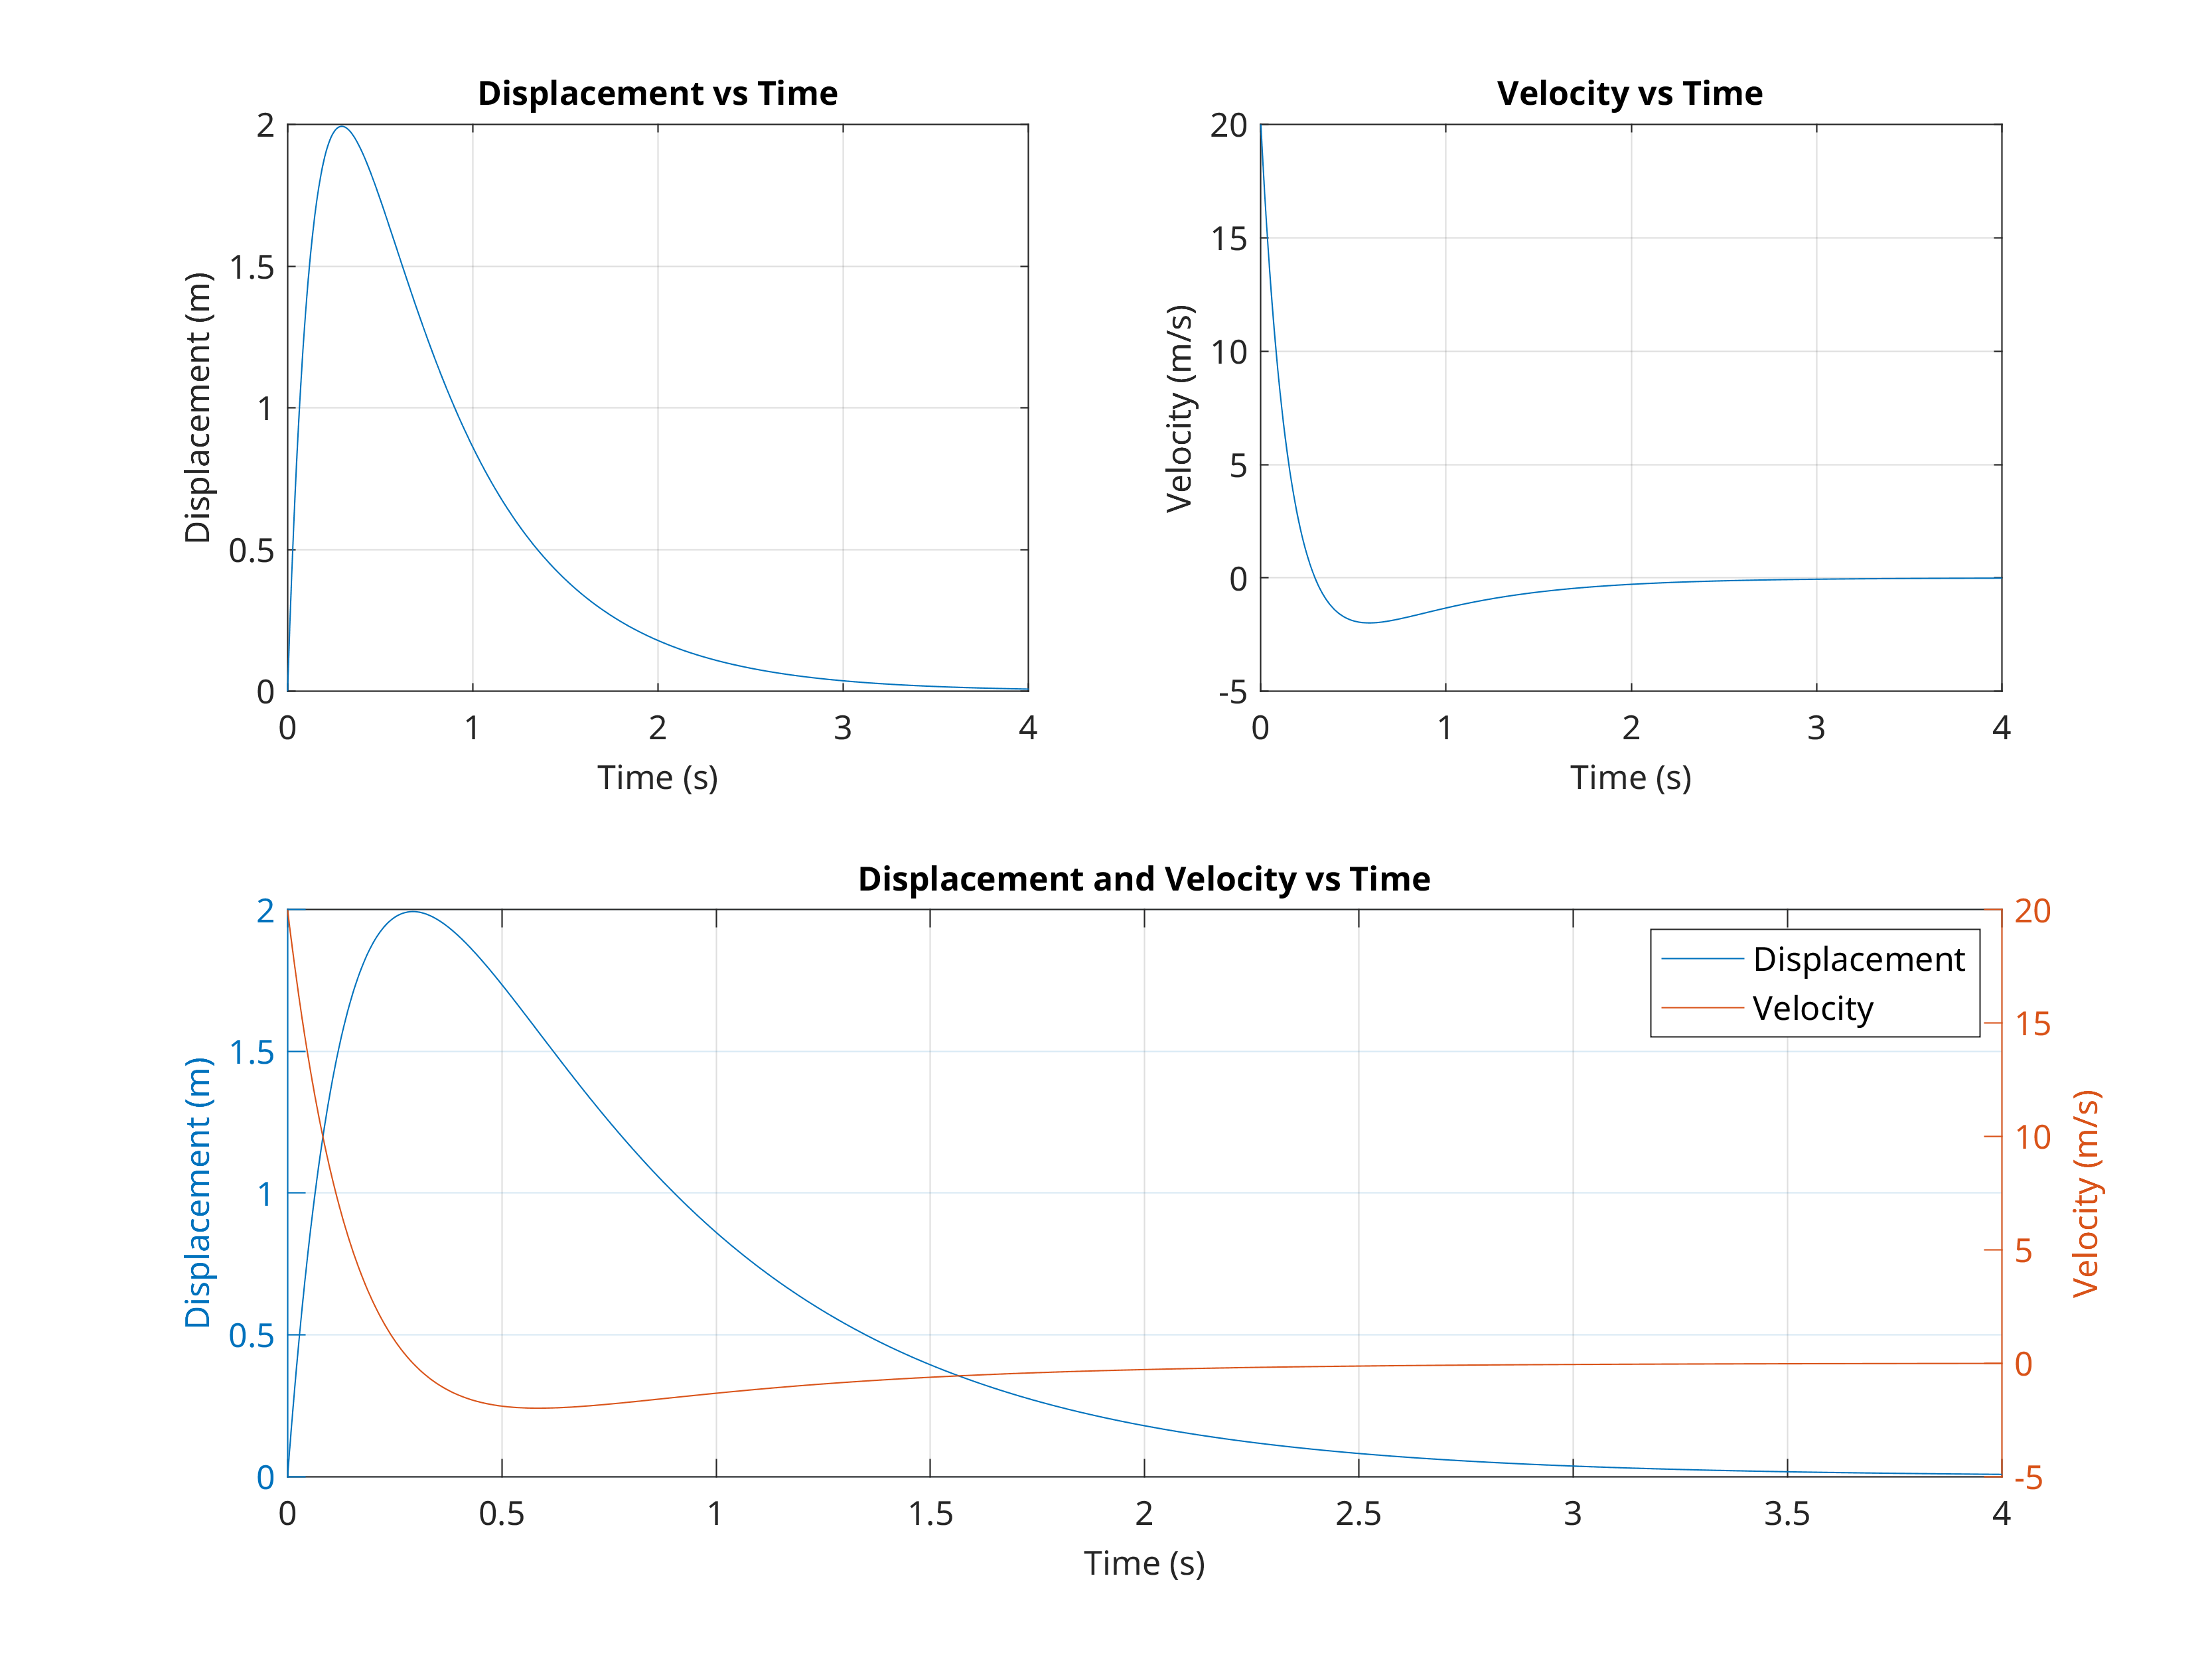
\includegraphics[width=1\textwidth]{images/railroad_bumper_plots.png}
    
    \newpage
    
    \begin{tcolorbox}[title={\color{black}{\section{Q10}}}, colback=white, colframe=\ni, boxrule=1mm, width=1\textwidth]    
        Aircraft A is flying east at \( 320 \, \text{mi/hr} \), while aircraft B is flying south at \( 160 \, \text{mi/hr} \).\\
        \centering
        
        At 1:00 p.m., the aircraft are located as shown.\\[15pt]
        
        
        \begin{tikzpicture}
            \draw[-] (0,0) -- (10,0);
            \draw[-] (8,3) -- (8,-3);
            \filldraw (1,0) circle (2pt) node[above=0.1cm] {A};
            \draw[line width = 0.4mm,-{Latex[length=2mm,width=2mm]}] (1,0) -- (2.4,0) node[above] {320 mi/h};
            \draw[-] (1,-0.3) -- (1,-1.7);
            \draw[{Stealth[length=2.5mm]}-{Stealth[length=2.5mm]}] (1,-1) -- (8,-1)  node[below, midway] {800 mi};
            \filldraw (8,2.2) circle (2pt) node[left=0.05cm] {B};
            \draw[line width = 0.4mm,-{Latex[length=2mm,width=2mm]}] (8,2.2) -- (8,1.4) node[above=0.1cm, left=0.1cm] {160 mi/h};
            \draw[-] (8.3,2.2) -- (9.7,2.2); 
            \draw[{Stealth[length=2.5mm]}-{Stealth[length=2.5mm]}] (9,2.2) -- (9,0) node[midway, right] {410 mi};
        \end{tikzpicture}\\[8pt]
        \raggedright
        \begin{itemize}[itemsep=-0.1cm]
            \item Obtain the expression for the distance \( D \) between the aircraft as a function of time \( t \).
            \item Plot \( D \) versus time until \( D \) reaches its minimum value.
            \item The plot must be of printing quality.
            \item Use the \texttt{roots} function to compute the time when the aircraft are first within \( 30 \, \text{mi} \) of each other.    
        \end{itemize}
    \end{tcolorbox}
    
    \textbf{Step 1: Setting Up the Position Coordinates}\\[1em]
    At 1:00 p.m., the initial positions of the two aircraft are as follows:\\
     Aircraft A is located 800 miles west of the vertical line where Aircraft B is positioned, and Aircraft B is 410 miles north of the horizontal line where Aircraft A is located.\\[1em]
    We assume that Aircraft A is flying east at a speed of \( 320 \, \text{mi/hr} \), while Aircraft B is moving south at \( 160 \, \text{mi/hr} \).\\[1em]
    Let \( t = 0 \) represent 1:00 p.m., the starting time. We denote the eastward position of Aircraft A at time \( t \) as \( x_A(t) \), and the southward position of Aircraft B at time \( y_B(t) \).\\[1em]
    
    \textbf{Step 2: Expressing Positions as Functions of Time}\\[1em]    
    
    \begin{minipage}{0.45\textwidth}\centering
        \textbf{Aircraft A's Position:} Since \textbf{Aircraft A} is moving eastward at \( 320 \, \text{mi/hr} \), given $(d=vt)$ its position \( x_A(t) \) relative to its starting point can be expressed as:
        \[x_A(t) = 320t\]
        Thus, the total horizontal distance from \textbf{Aircraft B} after \( t \) hours is:
        \[x(t) = 800 - x_A(t) = 800 - 320t\]
    \end{minipage}\hfil
    \begin{minipage}{0.45\textwidth}\centering
        \textbf{Aircraft B's Position:} Since \textbf{Aircraft B} is moving southward at \( 160 \, \text{mi/hr} \), given $(d=vt)$ its position \( y_B(t) \) relative to its starting point can be expressed as:
        \[y_B(t) = 160t\]
        Thus, the total vertical distance from \textbf{Aircraft A} after \( t \) hours is:
        \[y(t) = 410 - y_B(t) = 410 - 160t\]
    \end{minipage}\\
    
    \newpage

    \textbf{Step 3: Deriving the Distance \( D(t) \) Between the Aircraft}\\[1em]
    Using the Pythagorean theorem, the distance \( D(t) \) between the aircraft is:
    \[D(t) = \sqrt{x(t)^2 + y(t)^2}\]
    Substituting for \( x(t) \) and \( y(t) \):
    \[D(t) = \sqrt{(800 - 320t)^2 + (410 - 160t)^2}\]\\
    \vspace{1em}
    \begin{minipage}{0.45\textwidth}\centering
        \textbf{Computing the Time When Aircraft Are Within 30 Miles}\\[1em]
        To find when the aircraft are first within \( 30 \, \text{mi} \) of each other, set \( D(t) = 30 \) and solve for \( t \):
        \[30 = \sqrt{(800 - 320t)^2 + (410 - 160t)^2}\]
        Squaring both sides:
        \[900 = (800 - 320t)^2 + (410 - 160t)^2\]
        This equation can be simplified and solved using a computational tool such as MATLAB’s \texttt{roots} function.
    \end{minipage}\hfil
    \begin{minipage}{0.44\textwidth}\centering
        \textbf{Determining the Minimum Distance}\\[1em]
        To find the time \( t \) at which the distance \( D(t) \) reaches its minimum, we can take the derivative of \( D(t) \) with respect to \( t \), set it to zero, and solve for \( t \).\\[1em]
        However, since this expression is not needed to differentiate manually, we can use numerical methods or computational tools to find this minimum.\\[1em]
    \end{minipage}\\[2em]
    
    \textbf{Summary}
    \begin{itemize}[itemsep=-0.1cm]
        \item \textbf{Expression for \( D(t) \)}: The distance between the aircraft as a function of time is
        \[D(t) = \sqrt{(x_0 - V_A t)^2 + (y_0 - V_B t)^2}\]
        \item \textbf{Finding Minimum Distance}: Use MATLAB’s \texttt{min} function to find the minimum \( D(t) \) and the corresponding time \( t \).
        \item \textbf{Solving \( D(t) = 30 \)}: Set \( D(t) = 30 \) and use MATLAB’s \texttt{roots} function to find the time \( t \) when the aircraft are first within \( 30 \, \text{mi} \) of each other. we need in form of quadratic for \texttt{roots} function:
        \[0 = (V_A + V_B)t^2 - 2(V_A x_0 + V_B y_0)t + (x_0^2 + y_0^2 - 30^2)\]
        this yields the roots; using \texttt{min(root(coeff))} will give the first time the distance reaches \( 30 \, \text{mi} \).
    \end{itemize}

    \lstinputlisting[style=matlab, title=\textbf{\textcolor{\link}{\texttt{\href{https://github.com/sakx7/mathcompuni/blob/main/matlab scripts/q10.m}{matlab scripts/q10.m}}}}]{matlab scripts/q10.m}
    

    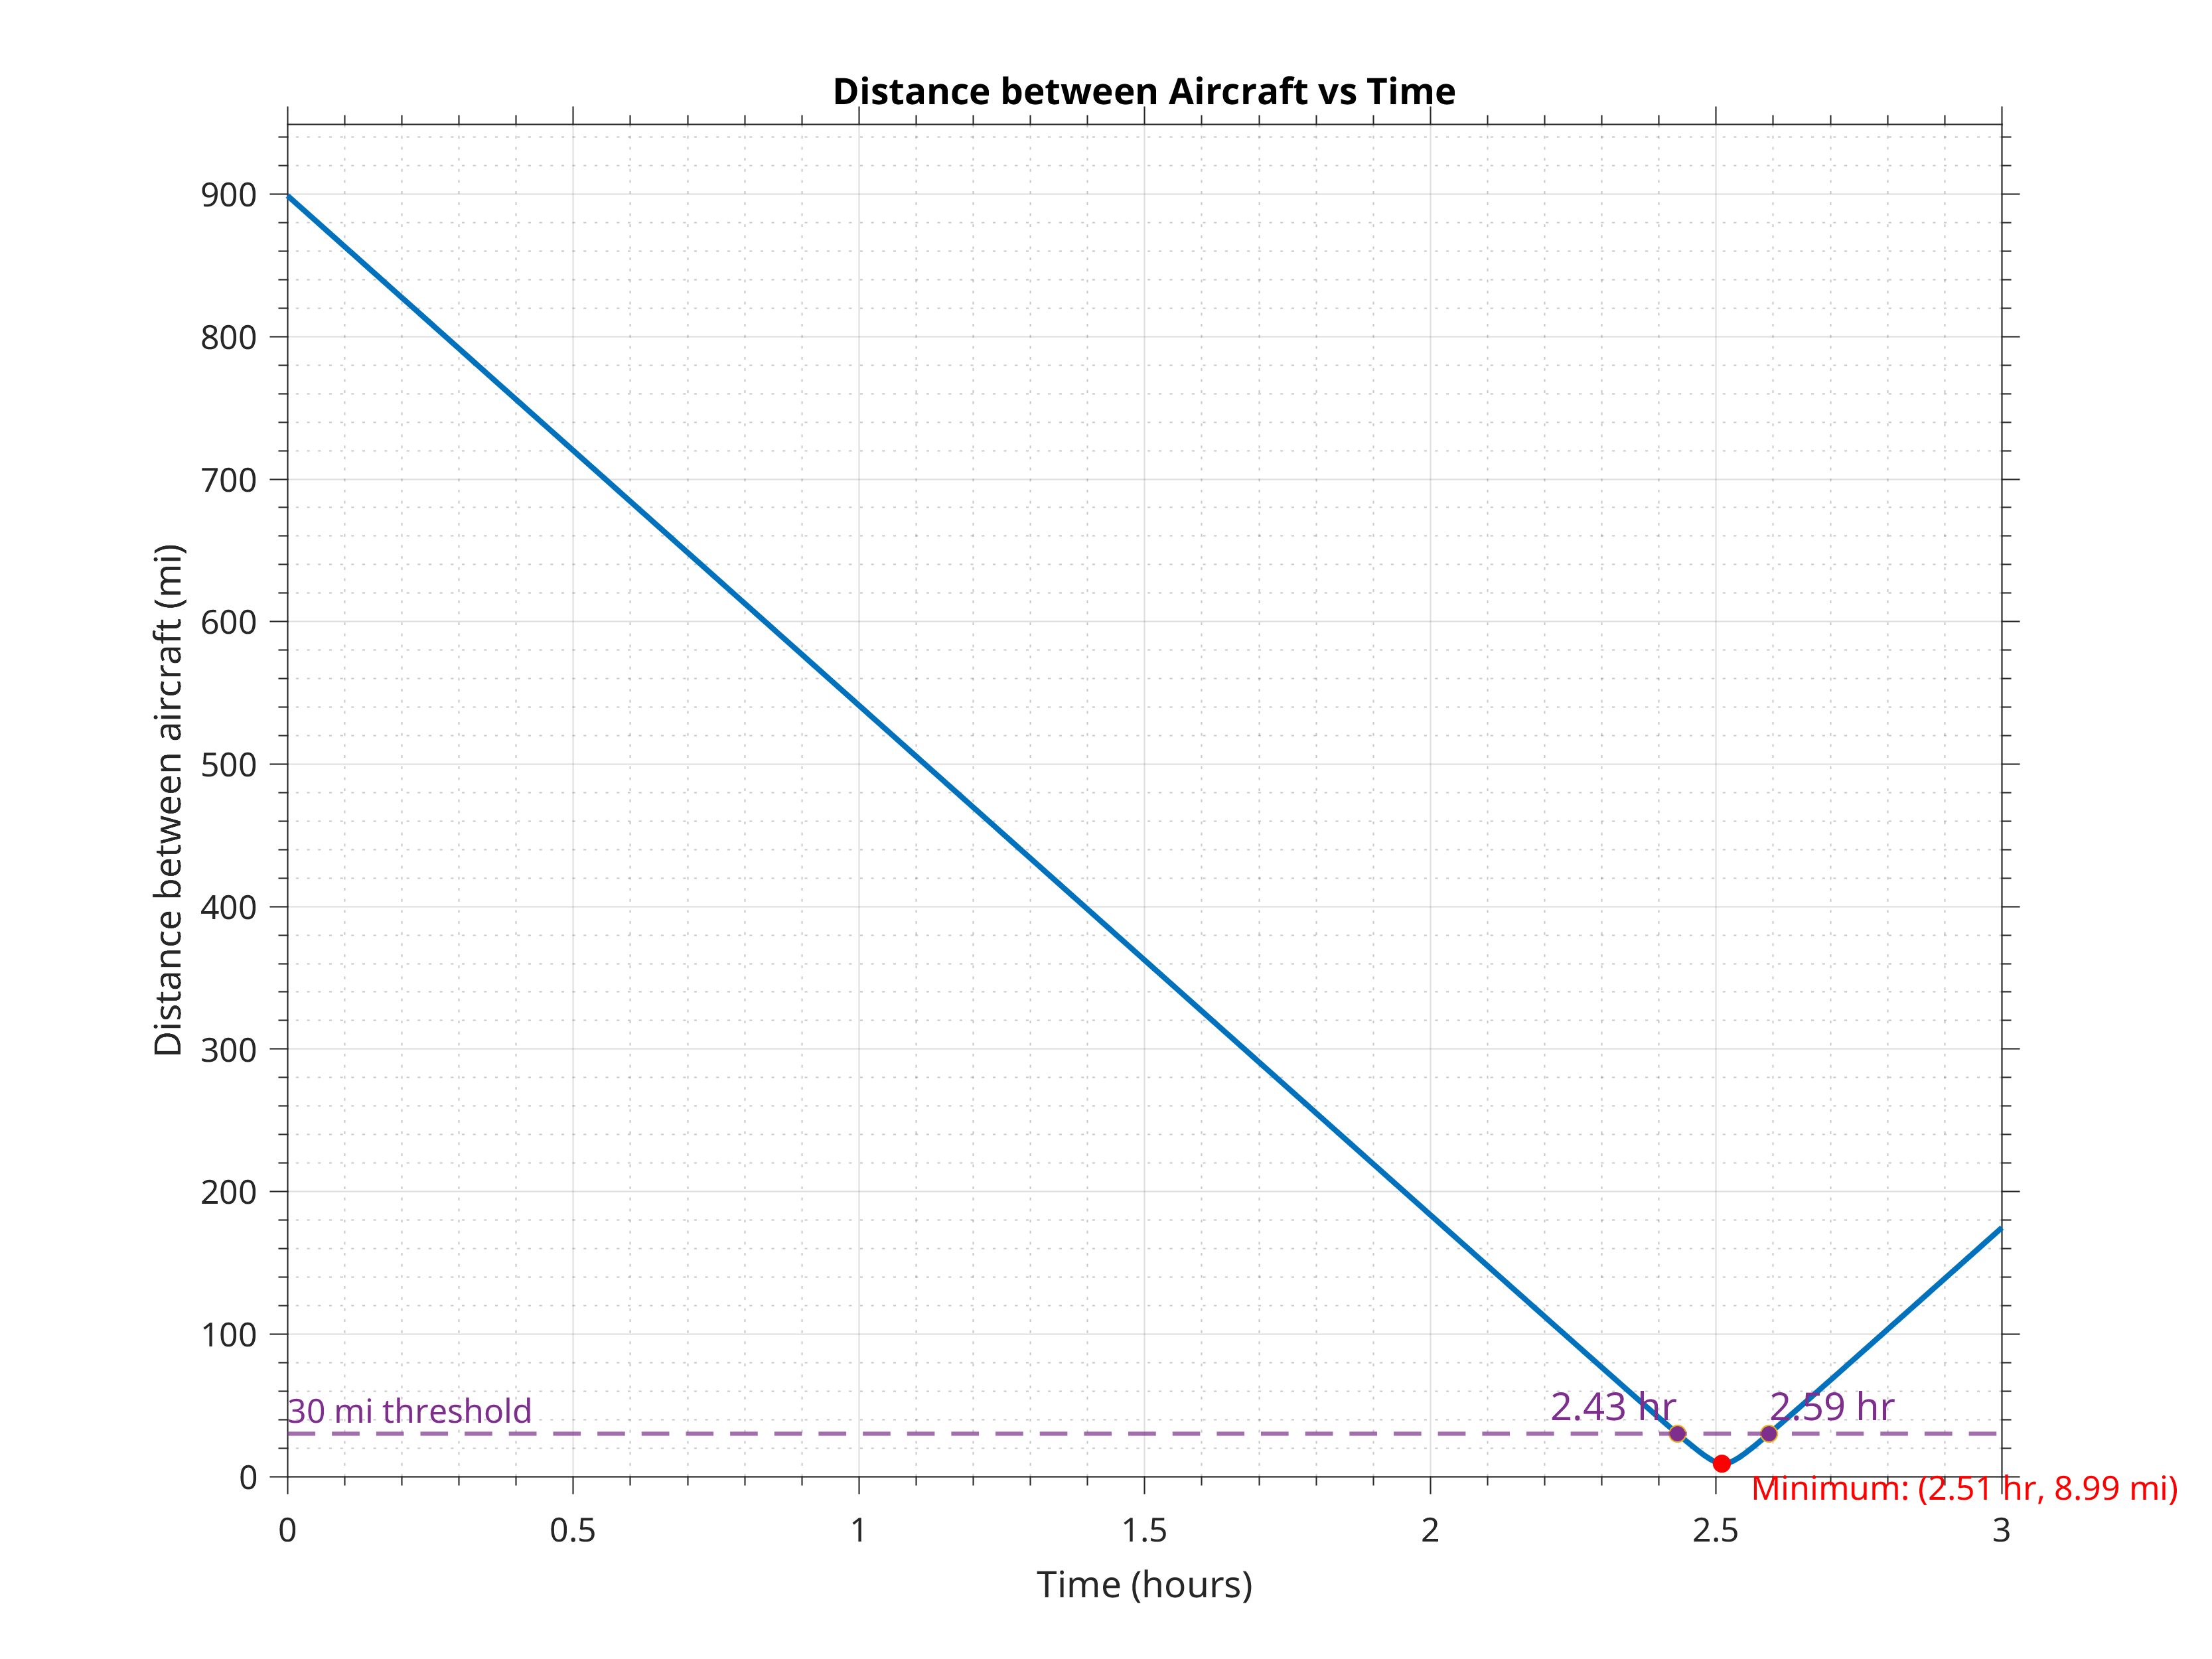
\includegraphics[width=1\textwidth]{images/aircraft_distance_plot.png}
    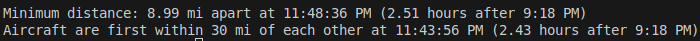
\includegraphics[width=1\textwidth]{images/q10.png}
    
    \newpage
    
    \begin{tcolorbox}[title={\color{black}{\section{Q11}}}, colback=white, colframe=\ni, boxrule=1mm, width=1\textwidth]    
        A two-dimensional state of stress at a point in a loaded material in the direction defined by the \( x - y \) coordinate system is defined by three components of stress \( \sigma_{xx} \), \( \sigma_{yy} \), and \( \tau_{xy} \). The stresses at the point in the direction defined by the \( x' - y' \) coordinate system are calculated by the stress transformation equations:
        \[\sigma_{x' x'} = \frac{\sigma_{xx} + \sigma_{yy}}{2} + \frac{\sigma_{xx} - \sigma_{yy}}{2} \cos(2\theta) + \tau_{xy} \sin(2\theta)\]
        \[\sigma_{y' y'} = \sigma_{xx} + \sigma_{yy} - \sigma_{x'x'}\]
        \[\tau_{x' y'} = -\frac{\sigma_{xx} - \sigma_{yy}}{2} \sin(2\theta) + \tau_{xy} \cos(2\theta)\]
        where \( \theta \) is the angle shown in the figure.\\[8pt]
        Write a user-defined MATLAB function that determines the stresses \( \sigma_{x' x'} \), \( \sigma_{y' y'} \), and \( \tau_{x' y'} \) given the stresses \( \sigma_{xx} \), \( \sigma_{yy} \), and \( \tau_{xy} \), and the angle \( \theta \). For the function name and arguments, use 
        \[[\text{Strain}] = \text{StressTrans}(S, \theta)\]
        The input argument \( S \) is a vector with the values of the three stress components \( \sigma_{xx} \), \( \sigma_{yy} \), and \( \tau_{xy} \), and the input argument \( \theta \) is a scalar with the value of \( \theta \).\\[8pt]
        The output argument \text{Strain} is a vector with the values of the three stress components \( \sigma_{x' x'} \), \( \sigma_{y' y'} \), and \( \tau_{x' y'} \).
   \end{tcolorbox}
   
    \lstinputlisting[style=matlab, title=\textbf{\textcolor{\link}{\texttt{\href{https://github.com/sakx7/mathcompuni/blob/main/matlab scripts/q11.m}{matlab scripts/q11.m}}}}]{matlab scripts/q11.m}
    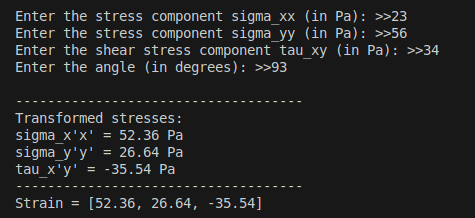
\includegraphics[width=0.6\textwidth]{images/q11.png}

\end{document}
